\documentclass{ieeeojies}
\usepackage{cite}
\usepackage{amsmath,amssymb,amsfonts}
\usepackage{algorithmic}
\usepackage{graphicx}
\usepackage{textcomp}
\usepackage{tabularx}
\usepackage{listings}
\usepackage{comment}
\usepackage{graphicx}
\usepackage{amsmath}
\usepackage{lineno}
\usepackage[linesnumbered,ruled,vlined]{algorithm2e}

\def\BibTeX{{\rm B\kern-.05em{\sc i\kern-.025em b}\kern-.08em
    T\kern-.1667em\lower.7ex\hbox{E}\kern-.125emX}}

\usepackage{soul}
\usepackage[normalem]{ulem}
\usepackage{comment}
\usepackage{xcolor}
\usepackage{listings}
\usepackage{tabularx}

\newcommand{\PreserveBackslash}[1]{\let\temp=\\#1\let\\=\temp}
\newcolumntype{C}[1]{>{\PreserveBackslash\centering}p{#1}}
\newcolumntype{R}[1]{>{\PreserveBackslash\raggedleft}p{#1}}
\newcolumntype{L}[1]{>{\PreserveBackslash\raggedright}p{#1}}
\definecolor{cred}{HTML}{FFB6B3}
\definecolor{cyellow}{HTML}{F7F4BA}
\definecolor{cgreen}{HTML}{E2F7DF}
\newcommand{\supported}{{\cellcolor{cgreen} $+$}}
\newcommand{\partially}{{\cellcolor{cyellow} $+/-$}}
\newcommand{\unsupported}{{\cellcolor{cred} $-$}}

%\newif\ifcomments
% comment out a different line to toggle comments
%\commentstrue
% \commentsfalse
\newcommand{\commentColor}[3]{\textcolor{#3}{[\textbf{#1:} #2]}}
\newcommand{\commentPO}[1]{\commentColor{PO}{#1}{teal}}
\newcommand{\commentVV}[1]{\commentColor{VV}{#1}{orange}}
\newcommand{\commentMX}[1]{\commentColor{MX}{#1}{brown}}

\newcommand{\PO}[1]{\textcolor{teal}{#1}}
\newcommand{\VV}[1]{\textcolor{orange}{#1}}
\newcommand{\MX}[1]{\textcolor{brown}{#1}}
\newcommand{\soutPO}[1]{\PO{\st{#1}}}
\newcommand{\corrPO}[2]{\soutPO{#1} \PO{#2}}

\newcommand{\etal}{\it et al. \normalfont}

%DIF PREAMBLE EXTENSION ADDED BY LATEXDIFF
%DIF UNDERLINE PREAMBLE %DIF PREAMBLE
\RequirePackage[normalem]{ulem} %DIF PREAMBLE
\RequirePackage{color}\definecolor{RED}{rgb}{1,0,0}\definecolor{BLUE}{rgb}{0,0,1} %DIF PREAMBLE
\providecommand{\DIFadd}[1]{{\protect\color{blue}\uwave{#1}}} %DIF PREAMBLE
\providecommand{\DIFdel}[1]{{\protect\color{red}\sout{#1}}}                      %DIF PREAMBLE
%DIF SAFE PREAMBLE %DIF PREAMBLE
\providecommand{\DIFaddbegin}{} %DIF PREAMBLE
\providecommand{\DIFaddend}{} %DIF PREAMBLE
\providecommand{\DIFdelbegin}{} %DIF PREAMBLE
\providecommand{\DIFdelend}{} %DIF PREAMBLE
\providecommand{\DIFmodbegin}{} %DIF PREAMBLE
\providecommand{\DIFmodend}{} %DIF PREAMBLE
%DIF FLOATSAFE PREAMBLE %DIF PREAMBLE
\providecommand{\DIFaddFL}[1]{\DIFadd{#1}} %DIF PREAMBLE
\providecommand{\DIFdelFL}[1]{\DIFdel{#1}} %DIF PREAMBLE
\providecommand{\DIFaddbeginFL}{} %DIF PREAMBLE
\providecommand{\DIFaddendFL}{} %DIF PREAMBLE
\providecommand{\DIFdelbeginFL}{} %DIF PREAMBLE
\providecommand{\DIFdelendFL}{} %DIF PREAMBLE
\newcommand{\DIFscaledelfig}{0.5}
%DIF HIGHLIGHTGRAPHICS PREAMBLE %DIF PREAMBLE
\RequirePackage{settobox} %DIF PREAMBLE
\RequirePackage{letltxmacro} %DIF PREAMBLE
\newsavebox{\DIFdelgraphicsbox} %DIF PREAMBLE
\newlength{\DIFdelgraphicswidth} %DIF PREAMBLE
\newlength{\DIFdelgraphicsheight} %DIF PREAMBLE
% store original definition of \includegraphics %DIF PREAMBLE
\LetLtxMacro{\DIFOincludegraphics}{\includegraphics} %DIF PREAMBLE
\newcommand{\DIFaddincludegraphics}[2][]{{\color{blue}\fbox{\DIFOincludegraphics[#1]{#2}}}} %DIF PREAMBLE
\newcommand{\DIFdelincludegraphics}[2][]{% %DIF PREAMBLE
\sbox{\DIFdelgraphicsbox}{\DIFOincludegraphics[#1]{#2}}% %DIF PREAMBLE
\settoboxwidth{\DIFdelgraphicswidth}{\DIFdelgraphicsbox} %DIF PREAMBLE
\settoboxtotalheight{\DIFdelgraphicsheight}{\DIFdelgraphicsbox} %DIF PREAMBLE
\scalebox{\DIFscaledelfig}{% %DIF PREAMBLE
\parbox[b]{\DIFdelgraphicswidth}{\usebox{\DIFdelgraphicsbox}\\[-\baselineskip] \rule{\DIFdelgraphicswidth}{0em}}\llap{\resizebox{\DIFdelgraphicswidth}{\DIFdelgraphicsheight}{% %DIF PREAMBLE
\setlength{\unitlength}{\DIFdelgraphicswidth}% %DIF PREAMBLE
\begin{picture}(1,1)% %DIF PREAMBLE
\thicklines\linethickness{2pt} %DIF PREAMBLE
{\color[rgb]{1,0,0}\put(0,0){\framebox(1,1){}}}% %DIF PREAMBLE
{\color[rgb]{1,0,0}\put(0,0){\line( 1,1){1}}}% %DIF PREAMBLE
{\color[rgb]{1,0,0}\put(0,1){\line(1,-1){1}}}% %DIF PREAMBLE
\end{picture}% %DIF PREAMBLE
}\hspace*{3pt}}} %DIF PREAMBLE
} %DIF PREAMBLE
\LetLtxMacro{\DIFOaddbegin}{\DIFaddbegin} %DIF PREAMBLE
\LetLtxMacro{\DIFOaddend}{\DIFaddend} %DIF PREAMBLE
\LetLtxMacro{\DIFOdelbegin}{\DIFdelbegin} %DIF PREAMBLE
\LetLtxMacro{\DIFOdelend}{\DIFdelend} %DIF PREAMBLE
\DeclareRobustCommand{\DIFaddbegin}{\DIFOaddbegin \let\includegraphics\DIFaddincludegraphics} %DIF PREAMBLE
\DeclareRobustCommand{\DIFaddend}{\DIFOaddend \let\includegraphics\DIFOincludegraphics} %DIF PREAMBLE
\DeclareRobustCommand{\DIFdelbegin}{\DIFOdelbegin \let\includegraphics\DIFdelincludegraphics} %DIF PREAMBLE
\DeclareRobustCommand{\DIFdelend}{\DIFOaddend \let\includegraphics\DIFOincludegraphics} %DIF PREAMBLE
\LetLtxMacro{\DIFOaddbeginFL}{\DIFaddbeginFL} %DIF PREAMBLE
\LetLtxMacro{\DIFOaddendFL}{\DIFaddendFL} %DIF PREAMBLE
\LetLtxMacro{\DIFOdelbeginFL}{\DIFdelbeginFL} %DIF PREAMBLE
\LetLtxMacro{\DIFOdelendFL}{\DIFdelendFL} %DIF PREAMBLE
\DeclareRobustCommand{\DIFaddbeginFL}{\DIFOaddbeginFL \let\includegraphics\DIFaddincludegraphics} %DIF PREAMBLE
\DeclareRobustCommand{\DIFaddendFL}{\DIFOaddendFL \let\includegraphics\DIFOincludegraphics} %DIF PREAMBLE
\DeclareRobustCommand{\DIFdelbeginFL}{\DIFOdelbeginFL \let\includegraphics\DIFdelincludegraphics} %DIF PREAMBLE
\DeclareRobustCommand{\DIFdelendFL}{\DIFOaddendFL \let\includegraphics\DIFOincludegraphics} %DIF PREAMBLE
%DIF COLORLISTINGS PREAMBLE %DIF PREAMBLE
\RequirePackage{listings} %DIF PREAMBLE
\RequirePackage{color} %DIF PREAMBLE
\lstdefinelanguage{DIFcode}{ %DIF PREAMBLE
%DIF DIFCODE_UNDERLINE %DIF PREAMBLE
  moredelim=[il][\color{red}\sout]{\%DIF\ <\ }, %DIF PREAMBLE
  moredelim=[il][\color{blue}\uwave]{\%DIF\ >\ } %DIF PREAMBLE
} %DIF PREAMBLE
\lstdefinestyle{DIFverbatimstyle}{ %DIF PREAMBLE
	language=DIFcode, %DIF PREAMBLE
	basicstyle=\ttfamily, %DIF PREAMBLE
	columns=fullflexible, %DIF PREAMBLE
	keepspaces=true %DIF PREAMBLE
} %DIF PREAMBLE
\lstnewenvironment{DIFverbatim}{\lstset{style=DIFverbatimstyle}}{} %DIF PREAMBLE
\lstnewenvironment{DIFverbatim*}{\lstset{style=DIFverbatimstyle,showspaces=true}}{} %DIF PREAMBLE
%DIF END PREAMBLE EXTENSION ADDED BY LATEXDIFF



\begin{document}


\title{A framework for the generation of monitor and  plant model from event logs using process mining for formal verification of event-driven systems}

\author{\uppercase{Midhun Xavier} \authorrefmark{1},
\uppercase{Victor Dubinin} \authorrefmark{2},
\uppercase{Sandeep Patil}\authorrefmark{1} \IEEEmembership{Member, IEEE}\uppercase{ and Valeriy Vyatkin}  \authorrefmark{1,3}
\IEEEmembership{Fellow, IEEE}}
\address[1]{Luleå University of Technology, Luleå, Sweden (e-mails: midhun.xavier@ltu.se, sandeep.patil@ltu.se)}
\address[2]{Independent researcher (e-mail: dubinin.victor@gmail.com)}
\address[3]{Aalto University, Helsinki, Finland}

\tfootnote{This work was sponsored in part by the Horizon Europe project Zero-SWARM funded by the European Commission (grant agreement: 101057083).}



\corresp{Corresponding author: Valeriy Vyatkin (e-mail: Valeriy.Vyatkin@aalto.fi).}

\linenumbers

\begin{abstract}

This paper proposes a method for the automatic generation of a plant model and monitoring using process mining algorithms based on recorded event logs. The behavioural traces of the system are captured by recording event logs during plant operation in either manual control mode or with an automatic controller. Process discovery algorithms are then applied to extract the logic of the process behaviour properties from the recorded event logs. The result is represented as a Petri net, which is used to construct the state machine of the plant model and monitor and is in accordance with the IEC 61499 standard.  The monitor is implemented as a function block and can be deployed in  real time   to trigger an error signal whenever there is a deviation from the actual process scenario. The plant model and controller are connected in a closed loop and are used for the formal verification of the system with the help of the 'fb2smv' converter and symbolic model checking tool NuSMV.


\end{abstract}

\begin{keywords} IEC 61499, Formal Verification, Plant Model Generation, Process mining
\end{keywords}

\titlepgskip=-15pt

\maketitle

\section{Introduction}

The adoption of the IEC 61499 \cite{iec61499part12012} Standard in Industry 4.0 to model distributed systems signifies a reliable and widely accepted approach \cite{dai2017discrete}. In the IEC 61499 standard, the distributed control system is expressed in terms of a network of function blocks (FB) executed in an event-driven way, while individual FBs are implemented as state machines \cite{dai2012redesign,lewis2001modelling,frey2006modeling} 
called Execution Control Charts (ECC).


The design of distributed control for systems is composed of several mechatronic components with complex interactions and is susceptible to design faults in the real system. In order to detect potential errors during run-time, monitors \cite{wenger2015behavioral,do2020towards} can be used as a monitoring technique. The monitor can observe the process sequence and provide an alert or even stop the process if it deviates from the expected process flow. The deployment of distributed control systems without proper verification can cause significant damage to system components. Simulation \cite{ hegny2010iec} is another widely used error-capturing method, This method does not guarantee the absence of errors in the system. 

Formal verification \cite{patil2015formal,blech2016comparison} can be utilized to identify errors in the designed system by using Computation tree logic (CTL) and linear temporal logic (LTL) specifications. The development of a formal model for the system requires the creation of models for both the plant and controller. While creating a formal model for the controller is relatively straightforward, modeling the plant can be complicated and it requires manual development. Formal verification \cite{cengic2010formal1} offers a more rigorous approach to verifying the correctness of distributed automation systems. The article \cite{ramdani2020rctl} introduces reconfigurable CTL, an extension of classical CTL, aimed at streamlining the formal verification process for complex reconfigurable discrete-event systems by reducing the number of properties needing verification through the classification and prioritization of properties based on dominance and equivalence relations. By computationally exploring a broad range of error-causing scenarios within the system, formal verification techniques can provide a more comprehensive analysis of potential errors than simulation-based methods.

The manual implementation of plant models \cite{hanisch2009one, hegny2010iec} is complex and time-consuming hence the automatic generation of plant models \cite{xavier2021plant, xavier2022plant}  helps in many cases. The plant model can be implemented by obtaining system information through the recording of event sequences that occur within the system. 


This study focuses on generating a monitor and a plant model by leveraging a process mining methodology on recorded event logs. While the monitor can be represented in different process model paradigms for the purpose of conformance checking, this study focuses on developing a monitor based on the IEC 61499 FB. Subsequently, this monitor is deployed to evaluate conformance.


The study addresses the challenge of classic process mining, which typically constructs a model of the entire system. In our approach, the focus is on developing a model specifically for the uncontrolled behavior of the plant, with the intention of later integrating it with the control model to create a closed-loop system model. This approach aligns with the requirements of discrete event system verification.



The paper is structured as follows:  Section \ref{rw} provides an in-depth literature review that compares the proposed approach with existing methods found in prior research. Section \ref{background} provides an overview of the foundational concepts of the Reference Model of Control/Sensor Events Sequencing and outlines the process of decomposing Petri nets into State Machine Components (SMCs). The workflow and potential use cases are detailed in Section \ref{workflow}. Section \ref{FSMfromEL} describes the process of Finite State Machine (FSM) generation from the event log, including the implementation of both the monitor and the plant model within IEC 61499 FBs. Section \ref{cs} offers a case study focusing on a pneumatic cylinder, presenting comprehensive results and analysis. Finally, Section \ref{cf} serves as the conclusion, summarizing the paper's findings and delineating future objectives.


\section{Related Work }
\label{rw}
\hfill 

IEC 61499 \cite{iec61499part12012} is an international standard for the design and implementation of industrial automation systems (IAS), particularly in the realm of distributed control systems.  Christensen et al. \cite{christensen2000design} introduced a model-driven approach for distributed control systems within the context of IEC 61499 systems. Providing a framework for modeling, designing, and deploying distributed control systems using a modular and event-driven approach. IEC 61499 is employed in industrial applications due to its enhanced modularity \cite{thramboulidis2013iec}, control logic reusability \cite{hegny2012towards}, flexibility in complex processes \cite{dai2015bridging}, and improved interoperability among automation components \cite{sunder2006usability}.

The paper \cite{vyatkin2009iec} describes how IEC 61499 standard itself ensures safety, but it is necessary to verify the system before its deployment to guarantee its reliability.  Hegny et. al \cite{hegny2010iec} presented  IEC 61499 based simulation framework for model-driven production systems development. While simulation is valuable for identifying bugs and assessing system behavior, it alone does not guarantee error-free operation. In \cite{blech2016comparison},  the comparison of formal verification approaches for IEC 61499 to enhance safety assurance is explained. Formal analysis of IEC 61499 applications \cite{cengic2010formal1, cengic2010formal2 } involves mathematically proving that the control system meets specified safety properties and requirements. By applying formal methods \cite{schnakenbourg2002towards,yoong2010modelling}, potential hazards and errors can be rigorously identified and corrected.



In \cite{ vyatkin2008closed, pang2009systematic}, systematic closed-loop modelling in IEC 61499 FBs and its  formal verification is presented. Closed-loop formal verification in IEC 61499, where the plant model and controller are connected in a closed-loop, is a better approach \cite{sinha2019survey, xavier2023formal} as it allows for the verification of system properties under realistic operating conditions, ensuring that the control system behaves correctly and safely in response to dynamic and unpredictable environmental changes \cite{ovsiannikova2023formal}.



In \cite{hanisch2009one}, the plant model is presented not only for simulation but also serves the purpose of formal verification. The paper \cite{malik2017emulation} presents an efficient approach wherein the plant model is constructed within an IEC 61499 FB, simplifying the integration of the controller and plant within a closed-loop system. The introduction of the fb2SMV tool \cite{fb2smv} facilitates the conversion of FB code into SMV format, enabling the verification of CTL or LTL specifications through NuSMV model checker \cite{cimatti2002nusmv}, thus streamlining the formal verification process. In  \cite{xavier2021cyber}, a plant model in IEC 61499 FB with non-deterministic transitions (NDT) is introduced for formal verification. While this method provides a more realistic means of implementing the plant model, it does entail manual work that is susceptible to errors and can be time-intensive. In our previous study\cite{xavier2021plant}, we proposed a semi-automatic plant model generation in SMV, but it posed challenges in integrating with the SMV model of the controller for closed-loop formal verification.



The research gap centers on the automatic generation of a plant model within IEC 61499 FBs to facilitate formal verification, and this paper aims to fill this void. In this study, we employ recorded events and leverage a process mining approach to develop a plant model. While process mining typically yields an overview of the entire system's behavior, this paper specifically details the extraction of the plant model using IEC 61499 FBs from this broader system behavior.



Process mining is a data-driven technique used to discover, monitor, and improve real-world processes by analyzing event logs and extracting valuable insights about how these processes are executed \cite{agrawal1998mining, van2012process1}. Beyond the realm of business process modeling, such methods are also applied in anomaly detection, cyber-attack detection, and alarm analysis within industrial control systems, utilizing a range of control flow discovery algorithms \cite{xavier2022process}. By analyzing event logs from various components and sensors, it can provide a comprehensive view of the system's operational behavior, enabling the identification of bottlenecks, deviations, and inefficiencies. This study applies similar principles to derive the process sequence of a controlled system, utilizing a mining algorithm for process discovery. ProM \cite{van2005prom} and DISCO \cite{gunther2012disco} are the widely used process mining tools for the preparation of event logs, process discovery, visualization, and conformance checking.  ProM \cite{ProM} which is used in this study, is an open-source tool, and comprises several process discovery algorithms and plugins for conformance checking and visualization. The \textbf{alpha} algorithm \cite{petri1962} is selected as the process discovery algorithm in this study due to its simplicity and transparency. Other process mining algorithms, such as the Heuristics Miner, Inductive Miner, or Genetic Miner are suggested when more complex or detailed insights are required \cite{dunzer2019conformance, naderifar2019review}. In recent research, process mining algorithms have shown the capability to handle multiple-concurrency short-loop structures effectively \cite{sun2021algorithm,sun2021process}. These algorithms can handle larger and more intricate event logs, making them suitable for in-depth analysis, optimization, and automation of processes. The selection of the algorithm should align with the objectives of the level of complexity in the process being analyzed \cite{xavier2022process}.



The study provides a comprehensive understanding of the system's behavior through event logs is available. This sets the stage for performing conformance checking  based on the model derived from these event logs \cite{van2012replaying, munoz2016conformance}.  This paper introduces a method for the automated generation of a monitor in IEC 61499 FBs, facilitating real time deployment for monitoring purposes. This IEC 61499 monitor FB analyzes all events to detect any deviations from the expected flow.  The combination of this monitor in the form of an IEC 61499 FB and the plant model represented similarly in IEC 61499 FBs becomes particularly advantageous when introducing new controllers or migrating to IEC 61499 FBs. The newly introduced controller can seamlessly connect in a closed-loop configuration with the plant model, and the developed IEC 61499 monitor FB allows us to monitor system behavior. Any deviation in events leading to an error state triggers the monitor, ensuring that the newly developed controller performs in accordance with the previous controller. The option to create a formal model of the system and perform formal verification adds an extra layer of safety assurance before deployment into the operational system.




\begin{figure*}[!t]
	\centering
	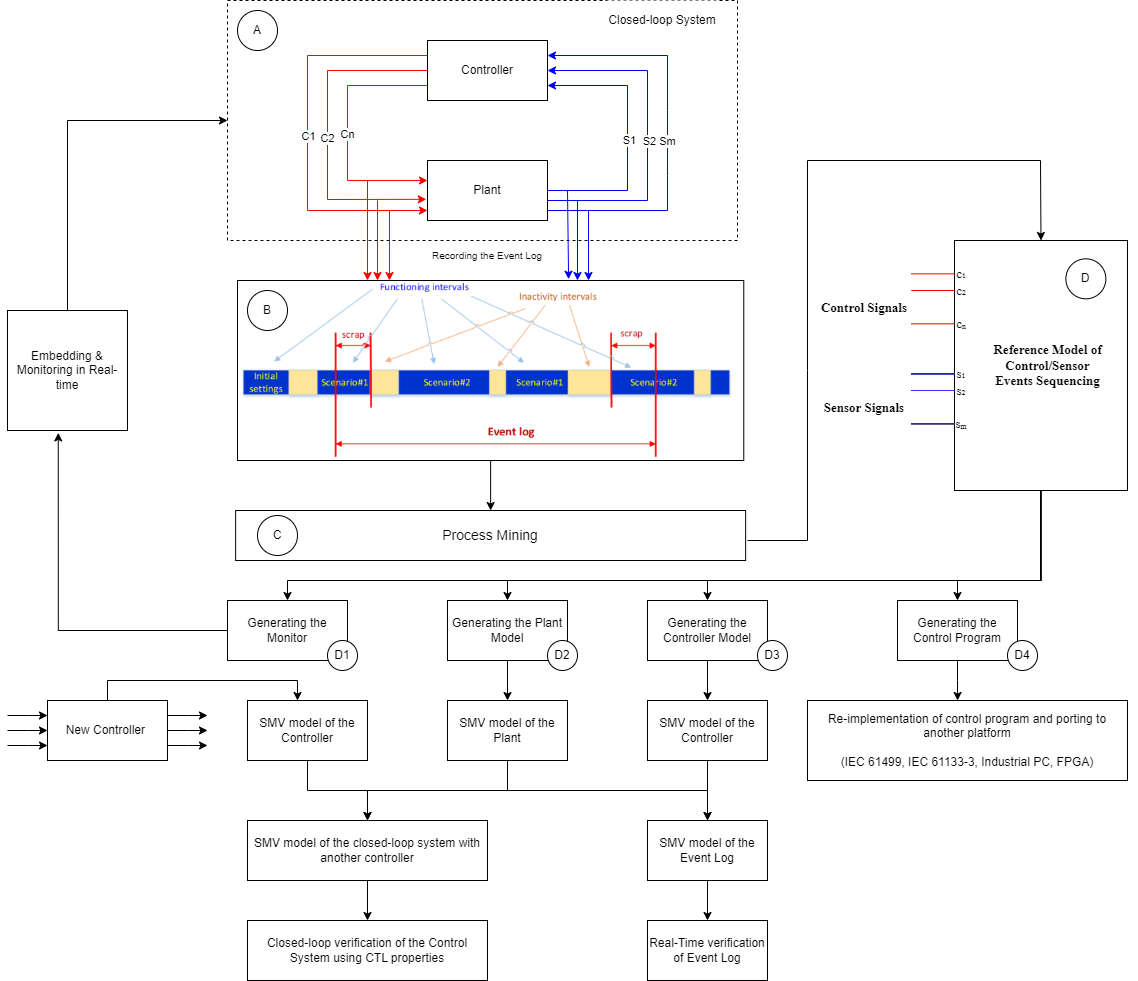
\includegraphics[width=0.9\textwidth]{images/workflow1.png}
	\caption{Workflow and use cases.}
	\label{workflowUsecase}
\end{figure*}

\section{Background}
\label{background}

\subsection{RMCSES Concept}
\label{rmcses}

The Reference Model of Control/Sensor Events Sequencing (RMCSES) is a formal model that developed from the process mining  \cite{cook1998discovering} of event logs describing the functioning of a closed-loop IAS in an "error-free" mode over an extended period. RMCSES offers a condensed representation of a vast event log, encompassing all possible signals from all components. Conceptually, if one imagines the event log as a collection of sentences or phrases of a formal language, describing the behavior of the IAS \cite{sinha2019survey}, then RMCSES functions as a sentence generator for this language. Due to its conciseness, RMCSES can be readily implemented in software or hardware.


The interface of the RMCSES is shown in Figure \ref{workflowUsecase} (D). The RMCSES only takes into account control signals originating from the controller and informative signals originating from sensors as events. These signals represent the interface between the controller and the plant. Internal signals circulating within the control system and the plant are not considered but it is possible to include control signals from external sources such as an operator.




In an IAS operating in an "error-free" mode, the functioning of each component is characterized by cyclical, meaningful, and locally complete processes. The insignificant operation of components, such as when an ejector piston moves back and forth indefinitely, is not considered. The component is identified to have meaningful behavior when it has a specific goal and actively works towards achieving it. Each component or device follows a specific scenario that begins with its initialization and ends with its termination. A multi-functional device may execute different scenarios depending on the specific task or operation it is performing.

Figure \ref{workflowUsecase}, (B) illustrates the cyclical operation of a component (device) and the possible cut-off points of the event log. As the functioning of a component (device) is cyclical, meaningful, and locally complete, the event log represents only a part of the process history of this component (device), leading to incomplete operation traces in the log that will be mapped onto the formal model. Therefore, a question arises as to how these incomplete traces, or "scraps," affect the extraction of an event log. Our experimental results indicate that the addition of such scraps to the event log does not result in significant changes.

Given the convenience of implementing the RMCSES as an IEC 61499 FB, we have opted to employ it as an FSM in our research; we do not preclude the use of alternative models. The RMCSES will constitute a comprehensive representation of the lower-level operation of the system; for intricate IAS, this model may become unwieldy.


%%As a rule, Petri nets \cite{van2013discovering} are used as a modeling formalism in Process Mining, since they are much more powerful than finite-automata (or, FSM) models. The state machine Petri net \VV{[REF?] - what is it?}} an be manually transformed using certain refactoring rules to a FSM representation and this approach is a practically “one-to-one” mapping into an ECC diagram of the basic FB. The goal of the refactoring is to get rid of constructs like "Fork into parallel branches" and "Join parallel branches" but such transformations are not always possible. 


Petri nets  \cite{van2013discovering} are frequently employed as a formalism for system modeling in the domain of process mining, as they offer greater expressive power in comparison to finite-automata models. The Petri nets are subsequently decomposed into SMCs and then composed to create an FSM through the application of specific refactoring rules. This FSM can be readily mapped onto an ECC diagram of a basic FB, with a near "one-to-one" correspondence. The primary goal of this refactoring procedure is to eliminate constructs such as "Fork into parallel branches" and "Join parallel branches". It should be noted that such transformations may not always be feasible.



\subsection{Overview of Petri net Decomposition Techniques}
\label{Petri net Decomposition}

Petri nets are essential for modeling concurrent systems \cite{liu2022petri} but can become complex as systems grow in scale. To manage this complexity, various decomposition techniques have been developed. These methods, including the Reachability Graph Method, Structural Decomposition Methods, and Linear Algebra-Based Methods, aim to break down Petri nets into more understandable components while preserving their essential behavioral characteristics. The Reachability Graph Method \cite{buchholz2002hierarchical} involves analyzing the reachability graph to identify subsets of states and transitions, facilitating the partitioning of the Petri net into manageable modules. Structural Decomposition Methods \cite{ye2017structural, hsieh2011robustness} leverage properties like perfect graph theory to systematically break down complex nets into simpler subnets. Linear Algebra-Based Methods \cite{wisniewski2019decomposition, best2013petri} use matrix manipulation to extract sequential components from place invariants, aiding in the identification of independent modules within the Petri net. These techniques offer distinct advantages in analyzing, verifying, and understanding concurrent systems modeled with Petri nets.


In this paper, the focus lies on accurately modeling a plant using IEC 61499 FBs to ensure the comprehensive capture of all its behaviors, vital for the proper functioning of the closed-loop system with a controller. To achieve this, the reachability graph \cite{miyamoto2013modular, giua1994petri} method is employed as a decomposition technique to derive SMCs from Petri nets. This method offers a structured and systematic approach to exploring all reachable states and transitions within the system, guaranteeing completeness in capturing all potential behaviors. By exhaustively mapping out all possible states and transitions, it ensures that no aspects are overlooked during analysis, providing a thorough understanding of the system's behavior dynamics and potential outcomes. It is susceptible to the state explosion problem \cite{kungas2005petri,buchholz2002hierarchical}, particularly in larger and more complex Petri nets, leading to computational inefficiency and difficulty in analysis. In contrast, structural decomposition methods leverage the Petri net's structural properties \cite{wisniewski2019analysis} to identify cohesive subsets that can be modeled as individual SMCs, providing flexibility in decomposition criteria. While these methods can offer more manageable representations and may be less prone to state explosion, their effectiveness heavily depends on the chosen structural properties and decomposition criteria, and may require domain-specific knowledge for optimal results. 

This paper discusses on the complete automatic generation of a plant model in IEC 61499 FB, identifying structural properties poses a challenge and necessitates domain-specific knowledge. Structural decomposition methods may offer a different approach by breaking down the system into smaller components based on structural properties \cite{kiviriga2023efficient}. This approach may overlook certain behaviors arising from interactions between components, unlike the comprehensive exploration provided by Reachability graphs. Reachability graphs provide a fine-grained analysis of the system's behavior, capturing individual states and transitions, which may be lacking in granularity in structural decomposition methods. Linear algebra-based methods \cite{wisniewski2014theoretical} provide a systematic approach to extracting sequential components from place invariants, offering insights into the structural properties of the Petri net. They may have limited applicability to Petri nets with complex or nonlinear dynamics and may be computationally intensive for large systems, requiring expertise in linear algebra \cite{cai1995modeling, wisniewski2019decomposition} for implementation and analysis. Overall, while the reachability graph method ensures completeness but suffers from state explosion, structural decomposition methods offer flexibility but depend on chosen criteria, and linear algebra-based methods provide insights but may have limited applicability and computational complexity, highlighting the trade-offs between completeness, flexibility, and computational efficiency in decomposing Petri nets into SMCs. 

Considering the trade-offs among different decomposition techniques, the need for completeness in capturing all system behaviors to ensure successful formal verification of closed-loop system properties is paramount. The challenge of state space explosion looms large, particularly in the Reachability graph method \cite{zambon2012graph, apel2016fly}. To address this, several strategies can be implemented \cite{xin2009methods}. State Space Reduction techniques involve the adoption of Symbolic Representations such as Binary Decision Diagrams (BDDs)  or Decision Diagrams to compactly represent sets of states \cite{shrestha2009decision}, thereby reducing memory requirements and mitigating state space explosion. A recent study \cite{he2022petri} presents an approach utilizing reduced ordered binary decision diagrams (ROBDD) to address state explosion issues in verifying privacy properties of multiagent systems modeled with knowledge-oriented Petri nets (KPNs) and computation tree logic of knowledge (CTLK), significantly reducing verification time even for large-scale systems such as the dining cryptographers protocol (DCP). Abstraction and Aggregation methods \cite{ludtke2018state} selectively abstract or aggregate unnecessary details in the reachability graph, focusing on essential behavioral properties while discarding less critical information, thus reducing the size of the state space and enhancing efficiency. Partial Order Reduction techniques \cite{godefroid1996partial, clarke1999state} aim to diminish redundant interleavings explored during state space traversal, avoiding the exploration of equivalent states and further reducing the size of the state space. clarke1999state,  a Hybrid Exploration Strategy is suggested. It involves Incremental Construction, where the reachability graph is dynamically constructed as needed during analysis, conserving memory and computational resources. On-the-Fly Exploration is employed to explore states as needed rather than generating all states upfront, efficiently managing state space explosion. Structural Decomposition techniques are integrated into the hybrid method, wherein the Petri net is decomposed into smaller subsystems, and reachability analysis is performed on each subsystem independently. This approach reduces the overall size of the state space that needs to be explored and analyzed, further mitigating state space explosion while ensuring comprehensive system behavior coverage.

Combining SMCs into a cohesive FSM necessitates careful integration to ensure synchronization and coordination between them. Several methods facilitate this process: Sequential Composition \cite{wisniewski2017prototyping}, where the output of one SMC becomes the input of another, suitable for systems with well-defined sequential behavior; Parallel Composition, involving concurrent execution of SMCs and combining their states and transitions to represent parallel behavior \cite{czerwinski2013finite}; Synchronization and Handshaking techniques \cite{cortadella2012logic} ensuring coordination between SMCs through protocols and clock domain crossing mechanisms; Global State Encoding \cite{el2006finite}, where individual SMC states are merged into a unified state space for comprehensive system representation; State Merging, identifying and collapsing equivalent states to manage complexity \cite{czerwinski2013synthesis}; and Interface Design and Refinement, establishing clear interfaces and refining interactions for modularity and maintainability. These methods offer practitioners a toolkit to effectively integrate SMCs, with choices guided by system characteristics like concurrency and synchronization needs, enabling the creation of a coherent FSM reflecting the overall system behavior.

For developing an FSM, a combination of parallel composition and synchronization techniques is preferred. Given the distributed nature and modularity requirements of IEC 61499 systems, parallel composition allows individual SMCs to represent concurrent activities effectively, aligning with the system's modular architecture. This approach facilitates easier maintenance, debugging, and resource utilization optimization. Synchronization techniques ensure proper coordination and communication between distributed SMCs, meeting real-time constraints and enhancing system correctness and reliability. By leveraging parallel composition and synchronization, developers can seamlessly integrate SMCs into a coherent FSM, enabling the development of robust and efficient ECC in IEC 61499 FB environments.

\section{ Workflow}
\label{workflow}


This section outlines the workflow and potential use cases enabled by RMCSES, as illustrated in Figure \ref{workflowUsecase}. Initially, signals from the distributed control system are recorded to construct RMCSES using process mining techniques. RMCSES then serves as the basis for generating the monitor (D1), plant model (D2), control model (D3), and control program (D4). In our prior research, we presented (D3) an interactive learning approach for deriving controller logic following the IEC 61499 standard \cite{xavier2022interactive}. Our previous study detailed (D2) the methodology and implementation of a basic plant model (a horizontal cylinder) \cite{xavier2022plant}. In this study, we enhance the methodology by incorporating global state information to create a precise plant model, subsequently closing the loop with a controller for formal verification using a toolchain \cite{xavier2021cyber}. Developing the monitor in IEC 61499 FBs is instrumental for real time error identification and prediction within the controller. In this paper, we develop such a monitor from event logs for conformance checking. Lastly, future work is planned to re-implement control and facilitate platform migration by deriving the control program from RMCSES.



\section{FSM from event logs and their implementation in IEC 61499 FBs}
\label{FSMfromEL}

This section describes the steps involved  in generating  IEC 61499 FBs from the recorded event log.

\begin{figure}[!t]
	\centering
	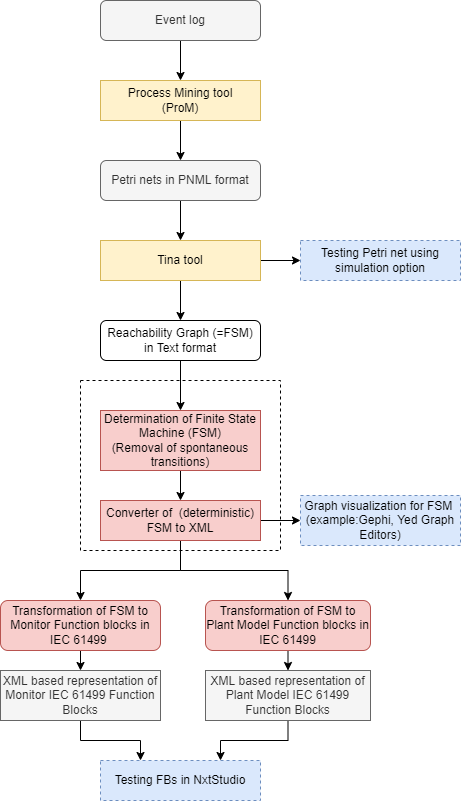
\includegraphics[width=0.4\textwidth]{images/Methodology.png}
	\caption{Tool chain and data flow for generating FSMs from Event Logs and their implementation in the form of IEC 61499 FBs.}
	\label{monitorFlowchart}
\end{figure}
    
\subsection{Petri net construction from event logs}



\begin{figure*}[!t]
	\centering
	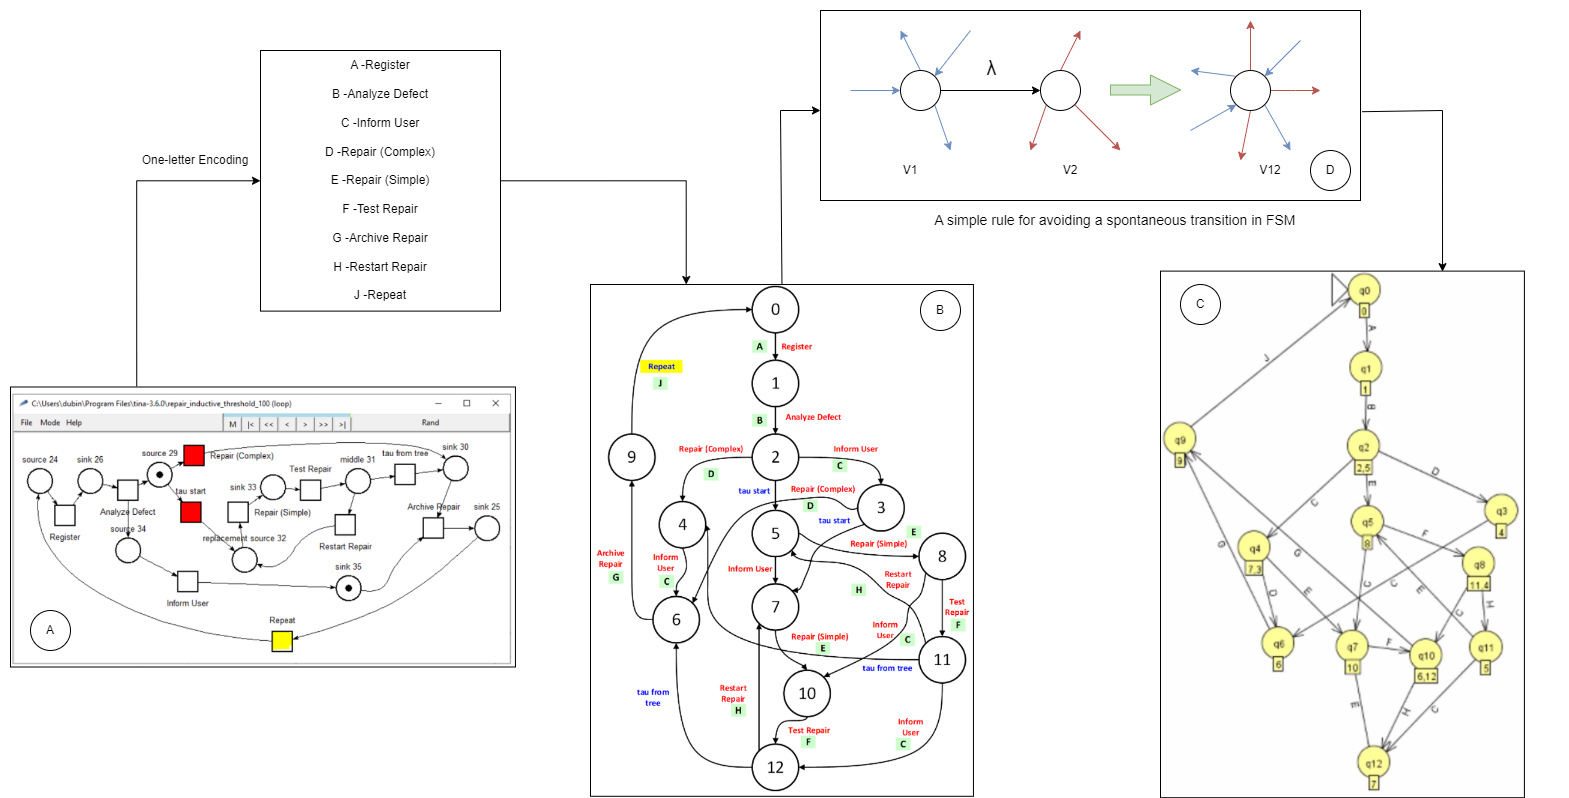
\includegraphics[width=1\textwidth]{images/PN2FSM.png}
	\caption{Transformation of Petri net to FSM for Monitor implementation.}
	\label{TR_PN2FSM}
\end{figure*}


The process of generating FSM from event logs and their implementation in the IEC 61499 FB is shown in Figure \ref{monitorFlowchart}. To start the process, the event log is given as input to the process mining tool called ProM \cite{ProM}, which is an open-source tool that offers various features such as representing process logic in different models, event log pre-processing, format conversion, conformance checking, LTL specification testing, and visualizations. The input event log is provided to ProM in CSV format, which then preprocesses the data and converts it into eXtensible Event Stream (XES) format. ProM then applies a process mining algorithm to the event log in XES format to extract processes in the form of Petri nets.


\subsection{ FSM generation from Petri net
}

\paragraph{From Petri Nets to SMCs: Utilizing Reachability Graphs for Decomposition}


To depict a Petri net within the ECC of IEC 61499 FBs, it's crucial to first decompose the Petri net into SMCss. Subsequently, these SMCs can be composed into a FSM.The extracted Petri net can be exported in the Petri net Markup Language (PNML) format using the ProM tool. The PNML-formatted Petri net is then given as input to the TINA tool  \cite{berthomieu2004tool}, which constructs a RG and can perform Petri net simulation. The finite RG is decomposed to SMC with spontaneous transitions as follows. 


Consider a running example "Repairing telephones" for the implementation of the IEC 61499 FB of the FSM for conformance checking. The description of the "Repairing telephones'' event log is given in ProM 6 tutorial, 2010 \cite{prom6tutorial}. The generated Petri net from the event log using an inductive miner is shown in Figure \ref{TR_PN2FSM} (A). A supplementary transition is added to the Petri net to make the process cyclic. In Figure \ref{TR_PN2FSM} (A), the Petri net is under stepwise simulation, and the 'Repeat' transition is added to make this process cyclic. Graphical representation of the RG is drawn manually using the RG text from TINA is outlined in Figure \ref{TR_PN2FSM} (B). The SMC is derived from the RG, and the transitions in the SMC are designated with the same names as the corresponding transitions in the Petri net. The "spontaneous" transitions are marked in blue color.


There appears to be a discrepancy regarding the potentially infinite nature of constructing a reachability set for a Petri net, which, in theory, could be infinite. It's essential to clarify that this set should not be infinite, as the event log, by its very nature, is finite. From a finite event log, a Petri net should indeed yield a finite number of reachable markings. The count of these markings should not exceed the number of entries in the event log, serving as an upper bound. This is grounded in the event log's representation as a very large RG with linear topology. Each event (entry) in the log distinctly defines a transition from one state (marking) to another. Modern tools for Petri net analysis can construct high-dimensional RGs, like those achieved through the Binary Decision Diagram (BDD) method. The challenge lies not in constructing the RG but rather in its implementation using IEC 61499 FBs. Nevertheless, even in cases where the RG comprises several thousand states, this challenge could be surmountable with the availability of appropriate CAD tools. It's worth noting that reduction methods for Petri nets may offer a viable strategy to significantly reduce the size of the RG, further enhancing the manageability of this complex process.

\paragraph{Tackling State Space Explosion: Effective Strategies for Petri Net Analysis}

Addressing the state space explosion issue in the reachability graph method for Petri nets involves employing various strategies to manage the exponential growth of states and transitions. Techniques such as abstraction and aggregation identify high-level patterns and structures for simplification, while partial order reduction reduces redundancy by exploring subsets of transitions together. Symmetry reduction exploits symmetrical properties to collapse equivalent states and transitions, effectively pruning redundant branches. On-the-fly exploration dynamically generates states and transitions only when needed, reducing memory consumption. State compression techniques compress state representations for efficient storage, and parallel and distributed exploration leverage parallelism to speed up analysis. By utilizing these methods, practitioners can navigate the complexities of larger Petri nets while efficiently managing computational resources, with the choice of approach guided by specific system characteristics and resource constraints.

\paragraph{Composing FSM from SMCs}
Developing a FSM from SMCs demands meticulous synchronization of decomposed components, a challenging task influenced by the system's clock domains. Within the framework of IEC 61499 FB, creating an ECC requires selecting an appropriate method for merging SMCs into an FSM, tailored to the specific requirements and characteristics of the distributed control system. The combined utilization of parallel composition and synchronization techniques emerges as the favored approach, offering concurrency management, modularity preservation, resource optimization, adherence to real-time constraints, and reinforcement of system correctness and reliability. These methodologies seamlessly align with the distributed and modular architecture of IEC 61499 systems, making them well-suited for consolidating SMCs into a coherent FSM.

To implement the strategy of parallel composition and synchronization techniques, the initial step involves identifying individual SMCs representing distinct functionalities within the distributed control system. Clear interfaces must be defined to delineate inputs, outputs, events, and communication protocols, facilitating seamless coordination among SMCs. Each SMC is then implemented as a separate module, enabling concurrent execution to handle various tasks efficiently. Event-driven communication serves as a pivotal synchronization mechanism, establishing communication channels between SMCs to facilitate information exchange and event triggering. Integration of SMCs into a unified system requires ensuring accurate interaction and synchronization based on defined interfaces and communication channels. Rigorous testing is essential to validate correctness, reliability, and real-time performance, with iterative refinement and optimization of the FSM to meet desired behavior and performance criteria. This approach, aligned with the distributed and modular nature of IEC 61499 systems, fosters the development of robust and efficient distributed control systems.

\subsection{Determinization of FSM with spontaneous transitions}

Non-determinism may occur in FSMs when employing "spontaneous" transitions within Petri nets. This means that the transitions of the Petri net are not related to any event. In the ProM system, they are indicated by black rectangles in Petri nets. The rule of mapping the transitions is as follows: A transition in an FSM  will be spontaneous if it corresponds to a "spontaneous" transition in the Petri net. In FSM, spontaneous transitions are denoted by the symbol $\lambda$  ("lambda")  or  $\epsilon$ ("epsilon").

The process of determinization can significantly simplify the implementation of a FSM in software. In this case, this process consists of getting rid of $\lambda$-arcs representing spontaneous transitions.


In this study, we use two approaches to the determinization of FSM that contain spontaneous transitions. The essence of the first approach is as follows: two vertices (states) connected by a $\lambda$-arc are combined into one vertex. In this case, the incoming and outgoing arcs of both vertices are combined, and the $\lambda$-arc is removed (see Figure \ref{TR_PN2FSM} (D) ). This rule is applied until there are no $\lambda$-arcs left in the transformed graph. This method is not universal and it is applicable only in the case of a tree-like topology of $\lambda$-arc relationships. In the second (universal) method, two vertices are contracted into one vertex if one vertex is reachable from another vertex through a chain of $\lambda$-arcs.


Determinization of an FSM can be omitted when there are no states with two or more spontaneous transitions outgoing from a state of the FSM. If there are no such situations, then a spontaneous transition can be interpreted in the ECC as a transition with an always true condition “1”.


\begin{figure*}[!t]
	\centering
	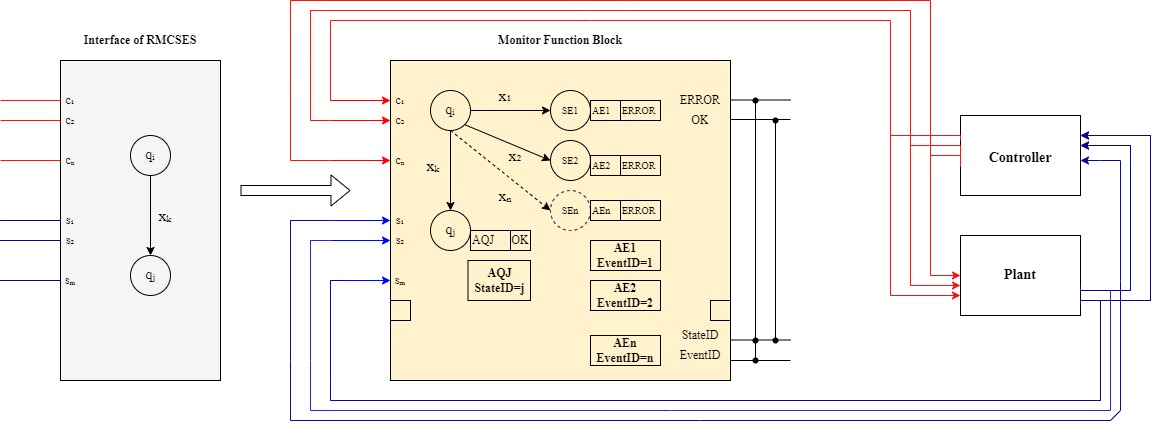
\includegraphics[width=1\textwidth]{images/ConformaceCheckingApp.jpg}
	\caption{Application for conformance checking.}
	\label{conformanceCheckingApp}

\end{figure*}


\subsection{Generation of Deterministic FSM }



The JFLAP tool \cite{rodger2015jflap} is used to implement the determinization of FSM. In this process, only one-letter designations of input symbols (signals) can be used. To encode the long names of input events used in the Petri net for the given example, we use a one-letter encoding (Figure \ref{TR_PN2FSM}).


The non-deterministic FSM  is shown in Figure \ref{TR_PN2FSM} (B), and spontaneous transitions are labeled with the symbol $\lambda$ (“lambda”). The transition labeled as J (i.e., "Repeat") from q9 to q0 will not take part in the determinization process. Instead, it will be replaced with the symbol "1" in the corresponding ECC. After determinization, the deterministic FSM is obtained as shown in Figure \ref{TR_PN2FSM} (C). GraphML format \cite{GraphMLSpec} was used to visualize the reachability graph with the  help of visualization tools like Gephi \cite{bastian2009gephi}, Yed \cite{yworks} etc. 

We employ a process discovery algorithm to generate a Petri net from the event log. Subsequently, we utilize the TINA tool to convert this Petri net into SMCs. This SMCs is further transformed into a deterministic FSM with the assistance of the JFLAP tool. These tools have gained widespread acceptance and are known for their accuracy and reliability in performing these conversions. By following this step-by-step approach and analyzing the model at each stage, we ensure the correctness of the transformation process. Attempting a direct conversion could be error-prone, making these integrated tools the preferred choice to prevent inaccuracies and streamline the workflow.




\subsection{Transformation of FSM to IEC 61499 FBs for monitor implementation}


The structure of the application for conformance checking is depicted in Figure \ref{conformanceCheckingApp}. The application is based on a closed-loop system that includes a plant and a controller. The RMCSES obtained from the event log is connected to the closed-loop system for the purpose of conformance checking. The RMCSES is implemented as a FSM that uses input data to drive its logic. The FSM is capable of detecting errors and verifying the correct sequence of steps in the process flow by monitoring events from the sensor and actuator in real time.







Figure \ref{conformanceCheckingApp} depicts the conversion of the RMCSES into the monitor. The monitor interface FB receives input signals in the form of controller signals $c_1 \dots c_n$ and sensor signals $s_1 \dots s_m$. The ECC is generated through the utilization of the transformation rule depicted in Figure \ref{conformanceCheckingApp}. An algorithm, based on this transformation rule and facilitating the conversion of FSM to ECC with error handling, is presented in Algorithm\ref{FSMtoMonitor}. When the monitor FB detects a valid transition from state $q_i$ to $q_j$ triggered by event $X_k$, it generates an output indicating a successful transition, denoted as "OK." If an unexpected event occurs, it transitions to the ERROR state, producing an ERROR event and providing details about the event that caused the error (EventID) and the StateID, which identifies the state where the error took place. This transformation rule ensures that the ECC reflects the behavior of the FSM  and is equipped to handle errors.





\begin{comment}
    

\subsubsection{Transformation of FSM to ECC with Error Handling}

\paragraph{ Define the FSM:} 

States: $\{q_1, q_2, \ldots, q_n\}$ \\
Inputs (events): $\{X_1, X_2, \ldots, X_m\}$ \\
Transitions: Represent transitions as a transition function  \\
$\delta: \text{States} \times \text{Inputs} \rightarrow \text{States}$, where $\delta(q_i, X_k) = q_j$ denotes a transition from state $q_i$ to $q_j$ when event $X_k$ is triggered.


\paragraph{Define the ECC:} 

States: $\{q_1, q_2, \ldots, q_n, \text{ERROR}\}$ \\
Inputs (events): $\{X_1, X_2, \ldots, X_m\}$ \\
Outputs (events): $\{\text{OK}, \text{ERROR}\}$ \\
EventID: An additional output to identify the last input event that caused an error.


\paragraph{Transformation Rule:}
 For each state $q_i$ in the FSM:
        \begin{itemize}
            \item If any event $X_k$ is triggered, create a transition in the ECC:
            \begin{itemize}
                \item ECC Transition: $(q_i, X_k) \rightarrow (q_j, \text{OK})$
            \end{itemize}
            This transition corresponds to a valid state transition in the FSM. State $q_j$ is reached, and the ECC outputs OK.
            
            \item For all other events $X_l \neq X_k$, create a transition to the ERROR state with additional outputs:
            \begin{itemize}
                \item ECC Transition: $(q_i, X_l) \rightarrow (\text{ERROR}, \text{ERROR})$
            \end{itemize}
            This transition represents an error state due to an unexpected event $X_l$. Additionally, set EventID to $X_l$ to indicate the event that caused the error.
        \end{itemize}


\end{comment}



\begin{algorithm}[t]
    \caption{FSM to Monitor ECC }
    \label{FSMtoMonitor}
\SetKwInOut{Input}{Input}
\SetKwInOut{Output}{Output}

\Input{ FSM = \{ Q: $\{q_0, q_1, \ldots, q_{n-1}\}$  
is a set of \\ states, where  $q_0$ is an initial state;\\
CS:  $\{X_1, X_2, \ldots, X_{p+r}\}$ 
is a set of input \\ symbols, where $X_i \in C \cup S$, where \\ C= $\{c_1,c_2,..., c_p\}$ is a set of control \\ signals, and S= $\{s_1,s_2,..., s_r\}$ is a set of \\ sensor signals; \\
$\delta \subseteq Q \times CS \times Q$ \} is a transition relation;
}
\Output{ ECC = \{ QC: $\{q_0, q_1, \ldots, q_{n-1}, {SE_n, SE_{n+1}} \dots {SE_{n+p+r-1}}\} \supset Q $ 
is a set of ECC states; \\
CS is a set of input events (see above);\\
Out: $\{\text{OK}, \text{ERROR}\}$  is a set of output events;\\
Alg= $\{a_0, a_1, \ldots, a_{n+p+r-1} \} $ is a set of \\ algorithms; \\ 
$\phi: \{ \text{Q} \times \text{CS} \rightarrow \text{QC} \times \text{Alg} \times \text{Out}$ \}  is an \\ ECC  transition function\} 

}
StateID=$q_0$  \\
{/* Creating the conforming (right) ECC transitions */}

\ForEach{$(q_i, X_k, q_j) \in \delta$ }{ 
Create ECC Transitions:
$(q_i, X_k) \rightarrow ( q_j, a_j, \text{OK})$
$a_j.StateID=j$  
} 

{/* Creating the non-conforming (erroneous) ECC transitions */}

\ForEach{$ q_w \in Q$ }{ 
\ForEach{$ X_e \in CS$ - $T(q_w)$}{ 
Create ECC Transitions:
$(q_w, X_e) \rightarrow (SE_e, a_e, \text{ERROR})$
$a_e.EventID=e$  
} 
} 
\Return{ECC}\; 

\textbf{ *Note* : Used variables and sets} \\

 StateID is an  output variable of the FB Monitor that stores the identifier of the current ECC  state;  \\

$a_j$.StateID is an occurrence of the  StateID  variable in the $a_j$ algorithm  associated with an ECC state;   \\

EventID is an  output variable of the FB Monitor that stores the identifier of the erroneous (not expected) input event; \\

$a_e$.EventID is an  occurrence of the EventID variable in the $a_e$ algorithm associated with an ECC state; \\

$T(q_w) \subseteq CS$ is a set of signals labelling the transitions outgoing from the ECC state $q_w \in Q$.

\end{algorithm}

\begin{figure*}[!t]
	\centering
	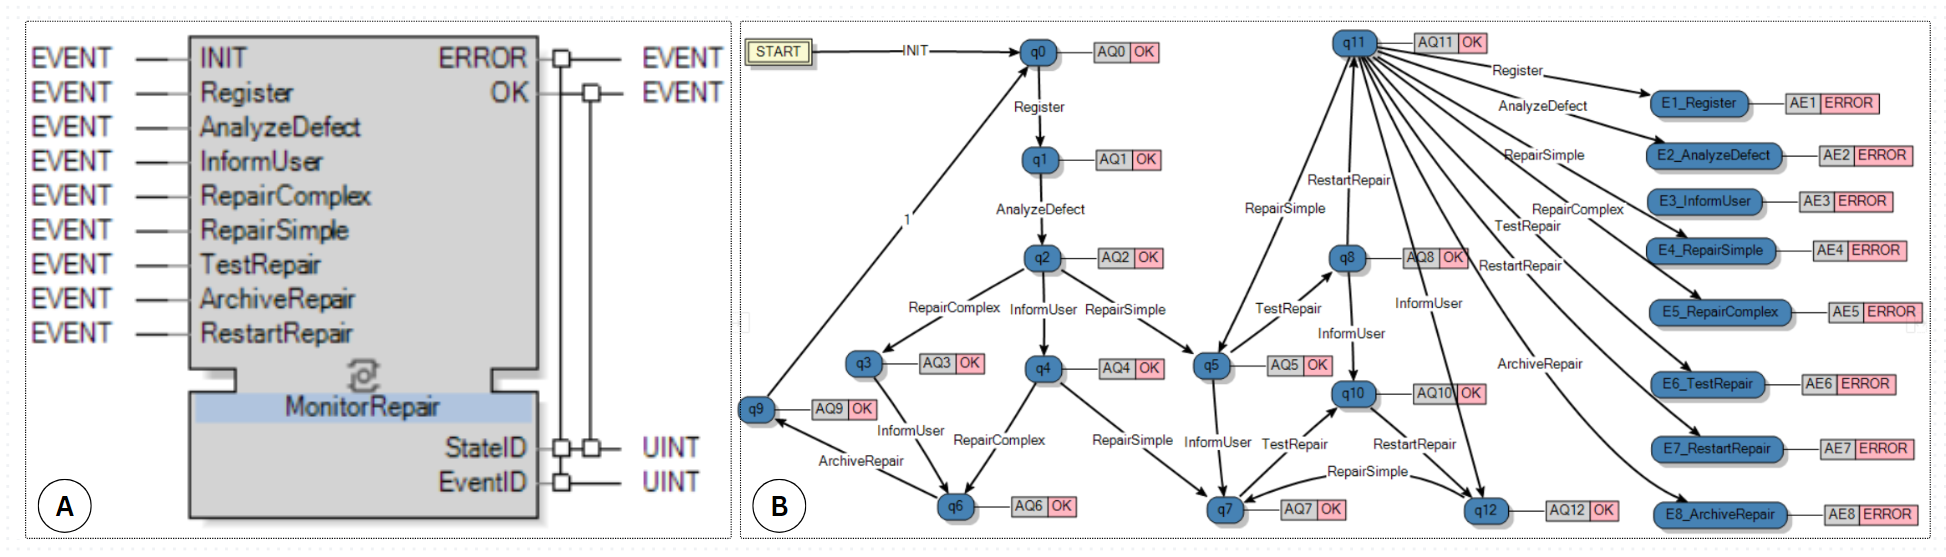
\includegraphics[width=1\textwidth]{images/MR.PNG}
	\caption{The FB interface and ECC of Telephone Repairing Monitor.}
	\label{TR_MonitorFB}
\end{figure*}

The Monitor FB shown in Figure \ref{conformanceCheckingApp}  is a direct implementation of the FSM, representing the formal reference model. The FSM is mapped to the ECC practically "one-to-one" and the FB interface is formed as follows. Each event is assigned its own event input. The INIT input signal is intended to set the model to the initial state. The signal from the event output 'OK' is issued when the received input event is in conformance with the formal reference model. In this case, the number (id) of the ECC state is issued, to which the transition took place (the output variable StateID). When an error is detected, not only the state number (StateID) where the error occurred but also the number of the input event (EventID) that led to the error is issued. Thus, the error is captured. The FB works until the first error appears, after that the FB is blocked. i.e., it becomes not responsive to any inputs. The ECC model is complete in the sense that from each basic ECC state, there are outgoing arcs labeled by each of the input events. Input events that are not specified for a state of the formal reference model transition the ECC to one of the error states. The ECC representation for the running example "Repairing telephones" is shown in Figure \ref{TR_MonitorFB} (B). For the sake of simplicity transitions to error, states are shown for only one test state q11.



It should be noted that the implementation of the monitor may differ in different tools. For example, in FBDK \cite{holobloc} it is simpler than in NxtStudio. This is due to the difference in execution models of basic FBs in these tools. While in FBDK the input event is immediately cleared after the activation (firing) of the ECC transition, in NxtStudio it is not cleared during the entire execution time of the FB (run-to-complete). As a result, during the execution of the FB, several ECC transitions marked with the same input event can be triggered.

\begin{comment}

Implementing the Monitor2 FB in FBDK is much simpler. In this case, the input interface of Monitor2 FB is the same as the input interface of Monitor1 FB. An error state is introduced, and the state transition diagram is augmented to be complete.

The implementation for NxtStudio is more complex. In this case, an additional event input must be introduced for each event input. For example, the \_Register (underlined) input event is introduced for the Register input event. "Normal" transitions between ECC states are marked with events without underlining, and transitions leading to an error state are marked with underscores. It is considered that all input events go in pairs - first there is an event without an underscore, and then an event with an underscore. Splitting the event into two is done outside the Monitor2 FB. When testing, one needs to click on two buttons in sequence, for example, first click Register button, and then \_Register button.
\end{comment}

\subsection{Extraction of plant model from the overall system model}

The FSM derived from the event log serves as a representation of the overall system behavior. In this study, an innovative approach for extracting the model of the uncontrolled plant is presented. The system is viewed as a closed-loop configuration, encompassing both the plant and the controller. The objective, therefore, centers on obtaining the model of uncontrolled plant behavior, which can subsequently be integrated with the control model, resulting in a closed-loop system model. This approach is particularly tailored to meet the requirements of event-driven system verification. The process of transitioning from the FSM to the plant model in the form of IEC 61499 FBs is elaborated upon below, illustrating our methodology for achieving this integration.

\subsection{Transformation of FSM plant model to IEC 61499 FBs }

\label{subsec:transformationOfFSMtoFB}

\begin{figure*}[!t]
	\centering
	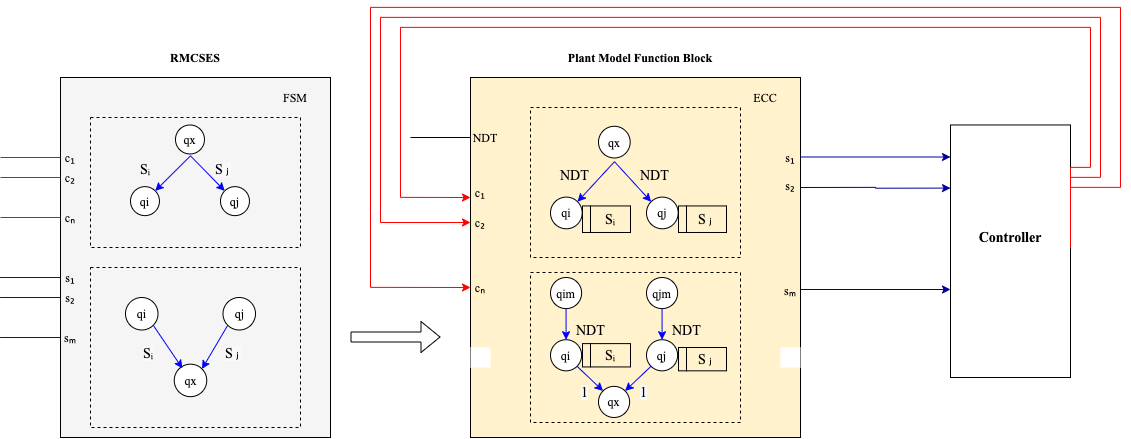
\includegraphics[width=0.9\textwidth]{images/VerificationApp1.png}
	\caption{Application for verification.}
	\label{verificationApp}
\end{figure*}


The presented application for verification follows a structure illustrated in Figure \ref{verificationApp}, where a closed-loop system is formed by connecting a plant model obtained from the RMCSES with either a new or an existing controller. An existing controller is utilized to construct the RMCSES, whereas a new controller is connected with RMCSES for the purpose of verification. The verification process involves conformance checking to ensure that the newly developed controller operates in accordance with the previous controller. NuSMV tool can be used for verification through CTL/LTL specifications.





\subsubsection{Transformation Rules from FSM to ECC }



The graphical depiction of the transformation of RMCSES to plant model in IEC 61499 FB is illustrated in Figure \ref{verificationApp}. The resulting plant model interface comprises control signals $c_1 \dots c_n$ and non-deterministic transitions (NDT) as input signals, while sensor signals $s_1 \dots s_m$ are designated as the output signals of the FB. In this transformation, any transition in the FSM triggered by a sensor signal is replaced by an NDT transition, with the output of the next state serving as a sensor event signal. This NDT serves as a mechanism for initiating transitions at arbitrary time intervals.  On the other hand, transitions within the FSM that are initiated by control signals remain unaltered when transitioning to the ECC model.




\paragraph{Case 1: Diverging Sensor Signals }



The transformation rule when sensor signal arcs diverge from a state is shown in Figure \ref{verificationApp}. When signals emanate from one state and branch out to multiple states, the sensor signals are substituted with NDT signals, and each output place generates the corresponding sensor signal as its output.



Given transitions in the FSM:


\[
\begin{aligned}
(q_x, s_i) & \rightarrow q_i \\
(q_x, s_j) & \rightarrow q_j \\
\end{aligned}
\]



In ECC, these transitions are replaced by NDT transitions with output events $s_i$ and $s_j$:



\[
\begin{aligned}
(q_x, \text{NDT}) & \rightarrow (q_i, s_i) \\
(q_x, \text{NDT}) & \rightarrow (q_j, s_j) \\
\end{aligned}
\]


\paragraph{Case 2: Converging Sensor Signals }



When signals come together into a single state from various states, they are altered according to the rule depicted in Figure \ref{verificationApp}. It's important to note that it's not feasible to bring multiple NDT signals together into the same state and generate two sensor signals as outputs. To address this, we introduced additional intermediary states that produce their respective sensor signals as outputs, and eventually, these states converge into a single state. The transformation rule for this scenario is as follows:



Given transitions in the FSM:
\[
\begin{aligned}
(q_i, s_i) & \rightarrow q_x \\
(q_j, s_j) & \rightarrow q_x \\
\end{aligned}
\]



In ECC, additional intermediate states $q_{im}$ and $q_{jm}$ are introduced, and NDT transitions are used to connect them to $q_i$ and $q_j$, respectively:


\[
\begin{aligned}
(q_{im}, \text{NDT}) & \rightarrow (q_i, s_i) \\
(q_{jm}, \text{NDT}) & \rightarrow (q_j, s_j) \\
\end{aligned}
\]


Finally, $q_i$ and $q_j$ converge to $q_x$:


\[
\begin{aligned}
(q_i, \text{1}) & \rightarrow q_x \\
(q_j, \text{1}) & \rightarrow q_x \\
\end{aligned}
\] 



\begin{algorithm}[t!]
    \caption{FSM to Plant model ECC }
    \label{FSMtoPlant}
\SetKwInOut{Input}{Input}
\SetKwInOut{Output}{Output}

\Input{ FSM = \{ Q: $\{q_0, q_1, \ldots, q_{n-1}\}$ \\
is a set of states, where $q_0$ is an initial state; \\
CS =  $ C \cup S$ is a set of input signals, where \\  C = $\{c_1, c_2, \ldots, c_p \}$ is a set of control \\  signals, \\  S = $\{s_1, s_2 \ldots, s_r \}$ is a set of sensorsignals; \\
$\delta \subseteq Q \times CS \times Q$ is a transition  relation; \}
}
\Output{ ECC = \{ $QC= Q \cup D$ is a set of ECC states, where D is a set of additional ECC states created dynamically;
$Cond= TC \cup \{1\}$ is a set of ECC transition  conditions, where $TC= C \cup \{NDT\}$ is a set  of input events;
S is a set of output events (see above);\\
$ \phi: QC \times Cond \rightarrow QC \cup QC\times S $ \\ is an ECC  transition function
\}
}

/* Processing the FSM transition labelled by control signals */

\ForEach{$(q_i, \sigma, q_j) \in \delta$}{
    \If{$\sigma \in $ C}{
        Create ECC Transition:
        $(q_i,  \sigma ) \rightarrow (q_j)$;\
    }
}
/* Processing the FSM transition labelled by sensor signals which are not converged */

\ForEach{$(q_i, \sigma, q_j) \in \delta$}{
    \If{$\sigma \in  S $ \text{AND}  $q_i \notin QJ$}{
        Create ECC Transition:
        $(q_i,  NDT ) \rightarrow (q_j, \sigma)$;\
    }
}

/* Processing the FSM transition labelled by converging sensor signals */

\ForEach{$(q_w \in QJ) $}{
\ForEach{$(q_i, \sigma, q_w) \in \delta$}{
    \If{$\sigma \in  S $}{
        Create ECC State $d \in D$ \\
        Create ECC Transition:
    $(q_i,  NDT ) \rightarrow (d, \sigma)$ ; \ \\
        $(d,  1 ) \rightarrow (q_w)$ ;\
    }
}

}
    \Return{ECC}\;

\textbf{ *Note* : Used variables and sets} \\
\BlankLine

$QJ= { \{ q_j \in Q , | \{(q_i, s_k, q_j) \in \delta’\}|>1} \} $, where $\delta’ = \delta \cap  Q \times S \times Q$ is a set of ECC states which have converging sensor signals in the FSM


\end{algorithm}

Algorithm \ref{FSMtoPlant} is defined by applying the transformation rules described earlier to facilitate the conversion of  RMSCES into a plant model in the IEC 61499 FB.


\subsection{MODEL-DRIVEN APPROACH AS A METHODOLOGICAL BASIS FOR DEVELOPMENT}

In this study, the model-driven approach (MDA) was used for development, according to which the design process is represented as a chain of model transformations, starting from the initial model and ending with the target one. In model-driven development the model transformation is “the heart and soul” of the approach \cite{sendall2003model}.
The event log as a source model, and the target models are: 1) the monitor model and 2) the plant model. In accordance with this, two different chains of transformations were used. The plant model is important as an independent result that can be used for various purposes in the design process, including certifying a new controller during transitions between different hardware and software platforms. This challenge of certifying is addressed in this study.
The certification process involves two essential activities: one is the creation of a model representing the plant through a series of transformations from event log to Petri net, RG, FSM of the plant, resulting in an IEC 61499 FB-based plant model. Next is the development of a comprehensive model for the new controller using IEC 61499 FBs. As the new controller is developed in IEC 61499 FBs, it is advisable to maintain consistency by expressing the plant model in the same notation. This design not only ensures uniformity but is also supported by the availability of the fb2smv, a tool that streamlines the conversion of IEC 61499 FBs into SMV code. These conversions, while intricate, are significant for systematic controller verification and migration, ensuring uniformity and reliability in the certification process. While many conversions are required primarily for certification and monitoring system implementation, a more direct approach is available when the sole goal is to verify an existing system based on event log data. In this scenario, the Petri net generated in ProM can be directly analyzed in dedicated platforms like TINA, which offers compatible tools for this purpose. There are different corresponding tools available within this system. There exist methods for directly converting Petri nets into SMV code \cite{wimmel1997bdd}. The resulting SMV code can be employed for analysis using queries rooted in LTL and CTL within systems like NuSMV.



\section{case study: A Pneumatic cylinder}
\label{cs}
\subsection{General Description}

Visualization of the cylinder's generated by its IEC 61499 simulation model in NxtStudio is shown in Figure \ref{VC_NXT_HMI}.  The cylinder has three sensors START, MID, and END indicating the position of the piston. The vertical cylinder's motion is controlled by EXT and RETR actuator signals'. EXT  to move downwards and RETR  to move upwards. The Actuator and Sensor signals of the pneumatic cylinder are represented in Figure \ref{VC_NXT_HMI}.


\begin{comment}
    

\begin{table}[]
    \centering
\begin{tabularx}{0.45\textwidth}  { 
   | >{\centering\arraybackslash}X 
  | >{\centering\arraybackslash}X 
  | >{\raggedleft\arraybackslash}X | }
  
 \hline
 Vertical cylinder Input & Vertical cylinder output\\
 Actuator signals & Sensor signals \\
 \hline
 Extend - EXT  & Position- START  \\
\hline
Retract -RETR  & Position- MID  \\
\hline
  & Position- END  \\
\hline
\end{tabularx}
    \caption{Actuator and Sensor signals of pneumatic cylinder}
    \label{tab:table1}
\end{table}
\end{comment}


\subsection{Event log Description}


The event log of the different processing scenarios of the vertical cylinder is recorded in CSV format, which captures the activities in chronological order. The event log, depicted in Figure \ref{EL2FSM} (A), comprises of three columns: CaseId, State, and Activity. The CaseId is unique for each processing scenario, while the Activity column represents the events that occurred during the processing of a scenario. Signals (like events) happen instantaneously, and it is a good practice to use the Boolean vector to store them, with "1" indicating it is set and "0" indicating it is reset. The timestamp information is used solely for sorting the activities in the event log.



\begin{figure}[!t]
	\centering
	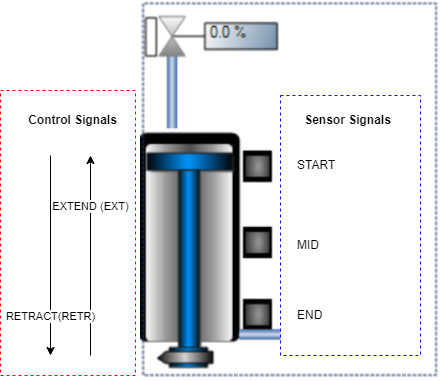
\includegraphics[width=0.35\textwidth]{images/CylinderHMI.png}
	\caption{Pneumatic cylinder HMI representation NXTSTUDIO.}
	\label{VC_NXT_HMI}
\end{figure}



\begin{figure*}[!t]
	\centering
	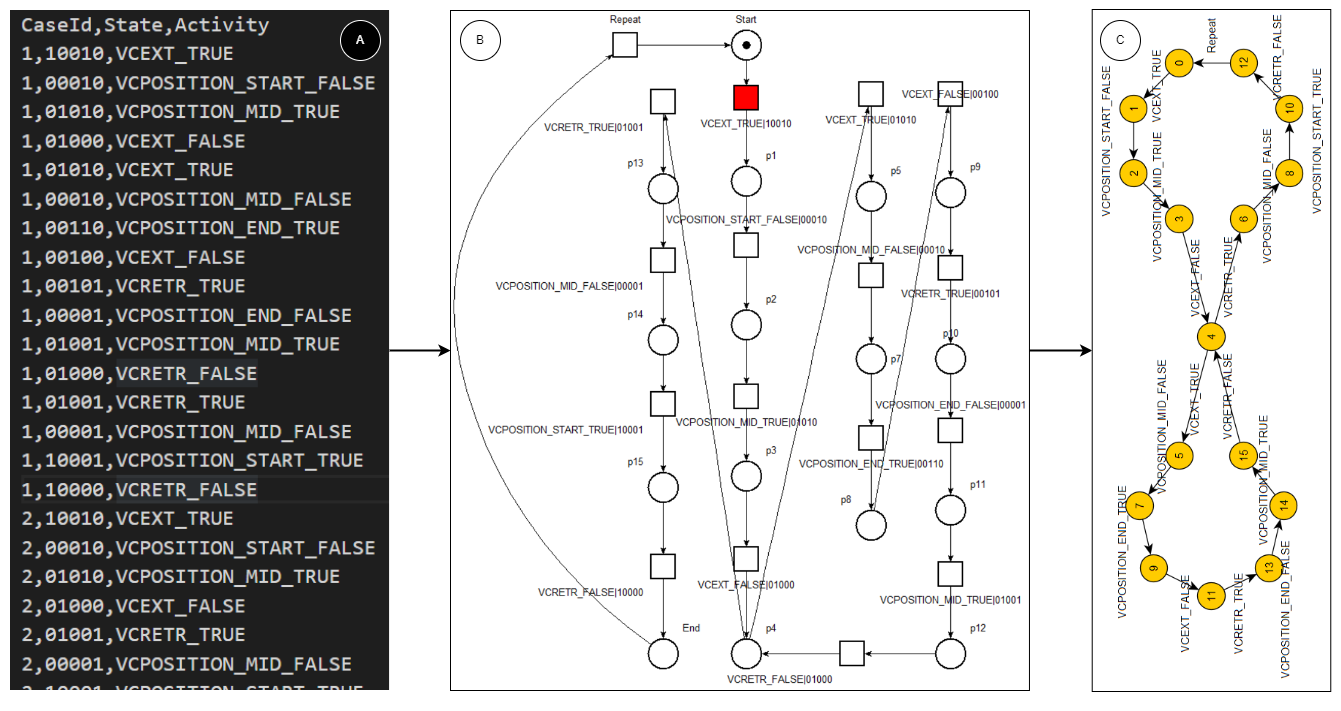
\includegraphics[width=1\textwidth]{images/EL2FSM.png}
	\caption{A) Vertical cylinder Event Log representation in CSV B) Stepwise simulation of Petri net in TINA C) FSM representation in Yed editor}
	\label{EL2FSM}
\end{figure*}


The event log captures various processing scenarios of the vertical cylinder, including movements from START to END via  MID,
  and returns to the START position. The event log also includes random movements of the cylinder captured by pressing the HMI buttons. These events are recorded using the OPC UA communication protocol.


\subsection{ FSM generation from event log}

The ProM process mining tool is utilized for constructing a Petri net from the event log. ProM offers several process discovery algorithms, and the \textbf{alpha} algorithm is utilized here for extracting the process from the event log. The event log, in CSV format, is first converted to XES format, and the 'Case' column is selected as 'CaseId', while the event column is a combination of 'Activity' and 'State' columns. This XES format is then provided as input to the alpha algorithm. The resulting Petri net is shown in Figure \ref{EL2FSM} (B).


The TINA tool is used to generate the RG for the Petri net. To achieve cyclic processing behavior, a new transition named 'Repeat' is added to the Petri net, connecting the 'END' state to the 'START' state. Stepwise simulation is performed to test the Petri net, as shown in Figure \ref{EL2FSM} (B). The RG is then used to generate the FSM in text format. The RG obtained from the Petri net can contain spontaneous transitions, rendering it a non-deterministic FSM. To convert this non-deterministic FSM to a deterministic one, the 'Converter of TINA RG to GraphML' software tool \cite{xavier2022interactive} is utilized. The resulting deterministic FSM is presented in Figure \ref{EL2FSM} (C) in GraphML format. The FSM is visualized using the 'Yed' GraphML editor \cite{yworks}, which provides a clear process logic behind the system. The state information on the edges of the FSM is removed since it is unnecessary to differentiate control and sensor signals.



\subsection{IEC 61499 representation of monitor}


\begin{figure*}[!t]
	\centering
	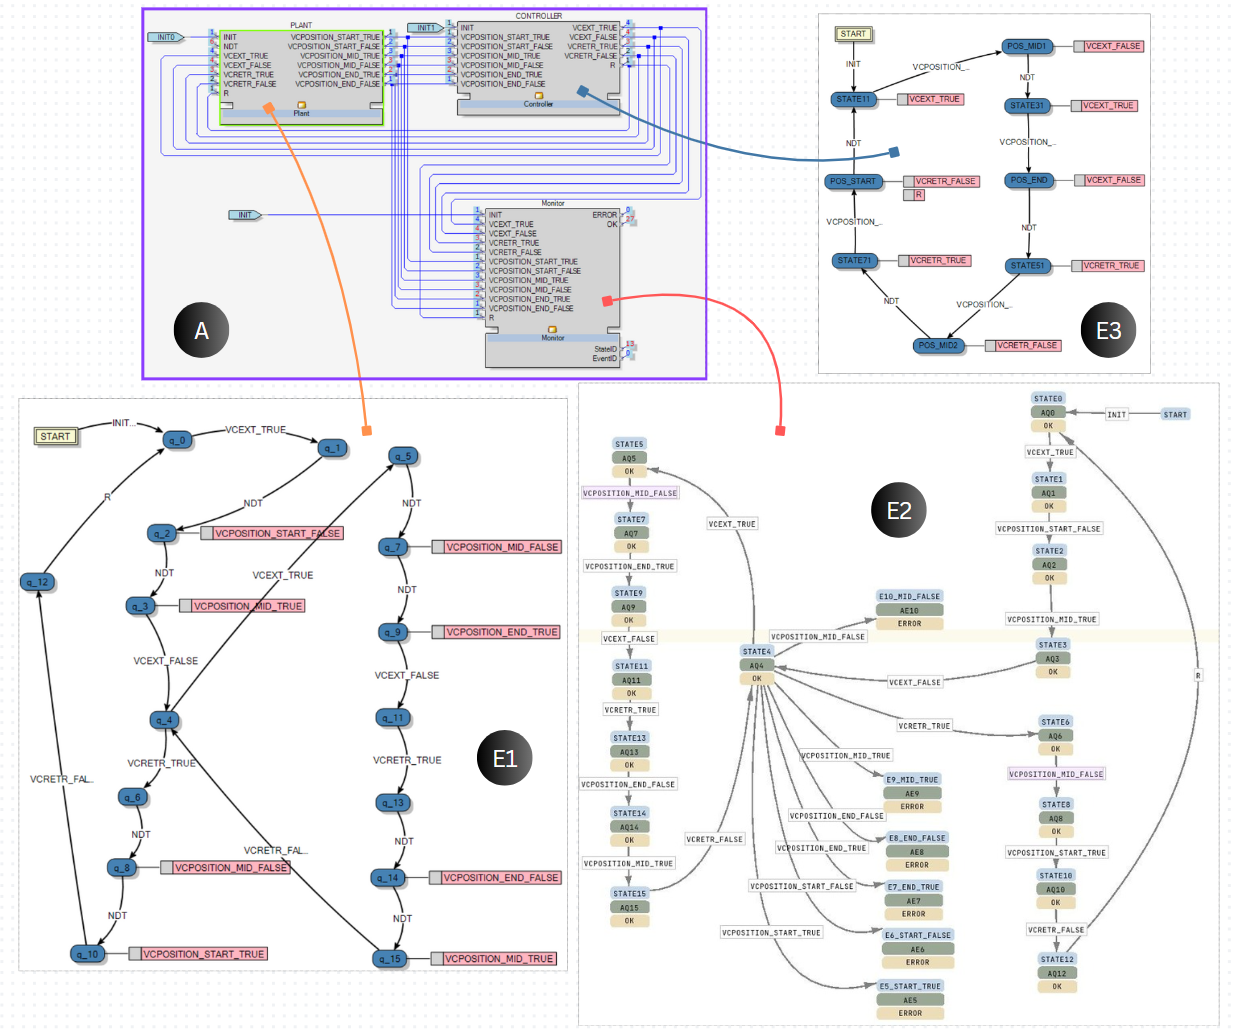
\includegraphics[width=1\textwidth]{images/CLMC.PNG}
	\caption{Closed-loop system of plant and controller model with the monitor.}
	\label{CL_plant_controller_monitor}
\end{figure*}


To implement the monitor in the IEC 61499 FBs, the RMCSES' FSM representation is taken as a starting point. The transformation rules are then applied to this FSM to create the monitor's FB interface. The interface, represented in Figure \ref{CL_plant_controller_monitor} (A), includes input signals for sensors and control signals. An additional event 'R' is included for the 'Repeat' event, which is used for the cyclic operation of the system's process.


The monitor FB generates an 'OK' event with the corresponding StateID when the system process executes in the correct order. In the case of any deviation from the expected process behavior, an 'ERROR' signal is emitted along with the 'EventID' indicating the specific event responsible for the deviation. The ECC for the monitor FB is represented partially in Figure \ref{CL_plant_controller_monitor} (E2). If any event other than 'VCEXT\_TRUE' and 'VCRETR\_FALSE' occurs in 'STATE4', an 'ERROR' event is triggered, along with the respective EventID. The ECC in Figure \ref{CL_plant_controller_monitor} (E2) only shows errors occurring from 'STATE 4', but in the actual scenario, there will be multiple events from different states (STATE1, STATE 2, etc.) leading to their corresponding ‘ERROR’ states (VCEXT\_TRUE, VCRETR\_FALSE, etc.).


\subsection{IEC 61499 representation of Plant Model}



The ECC of the plant model is generated using the deterministic FSM obtained from the Petri net. Transformation rules discussed in Section \ref{subsec:transformationOfFSMtoFB} are applied to the FSM to derive the ECC. The interface of the plant model mirrors the controller depicted in  Figure \ref{CL_plant_controller_monitor} (A). The plant model has an additional signal called NDT, which provides a non-deterministic delay before producing the sensor signals as output. The behavior of the system is represented by the ECC and is embedded inside a FB. The ECC of the plant model is illustrated in Figure  \ref{CL_plant_controller_monitor} (E1).


\section{Traces with only events, no global state}

\begin{figure}[!t]
	\centering
	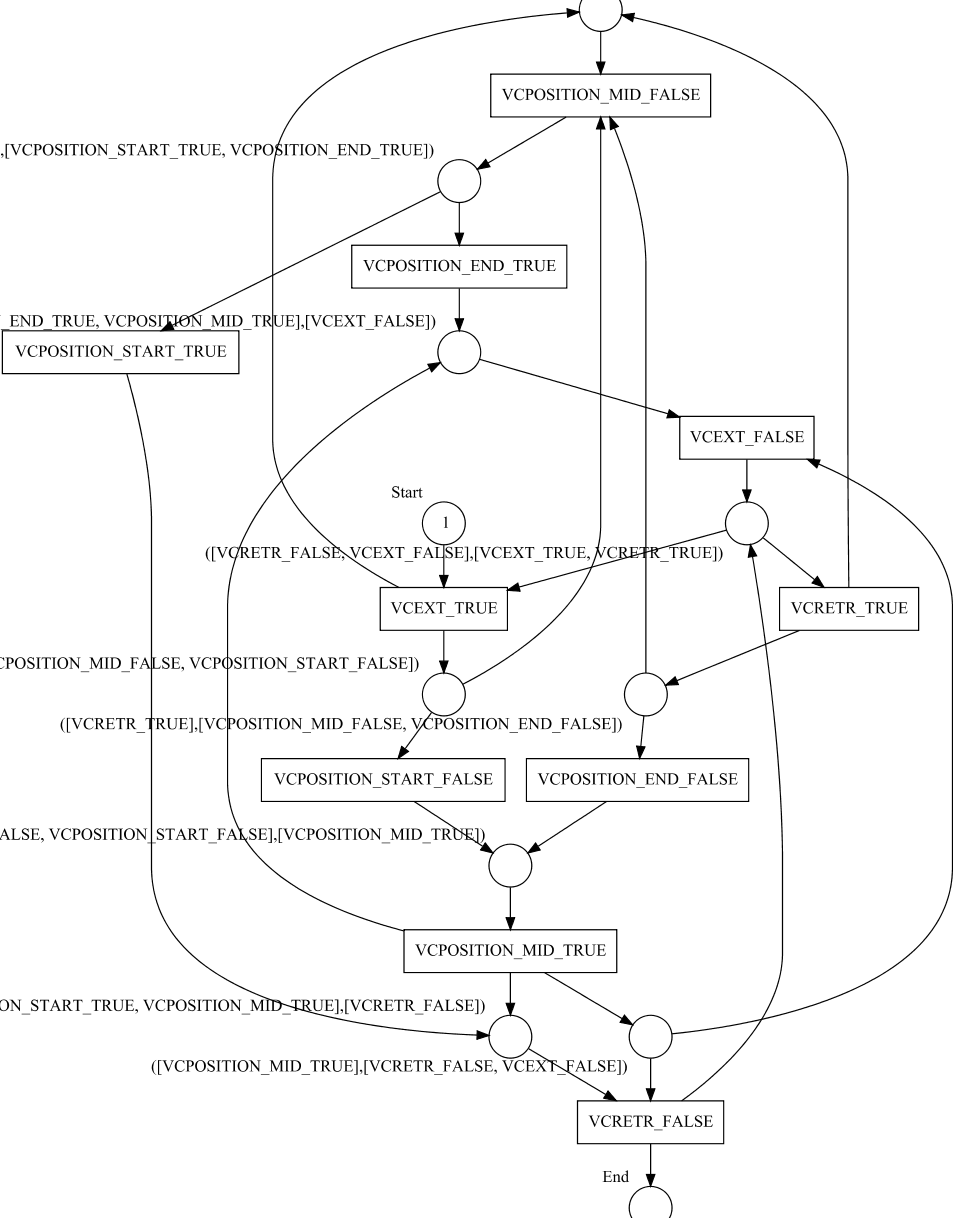
\includegraphics[width=0.4\textwidth]{images/StatelessPN.PNG}
	\caption{Petri net constructed without state information.}
	\label{StatelessPN}
\end{figure}

\subsection{Global state}


The global state of the system is defined as a vector of boolean values that represents the combination of sensor and actuator signals. This vector is used to construct the global state context of the system. The global state context represents a unique frame of reference for the system. To ensure the accuracy of the global state, clock synchronization and time stamping are used across all distributed controllers in the network.


\iffalse
The global state can be constructed relying on clock synchronization and time stamping.
What to do with big and linear state graphs?
Build state graphs using process mining without global state information.

Try to simulate it against the original traces and see if the entire graph is covered. 
If not, consider pruning the state graph.

Check the auto-generated model of the plant with another controller. 
\fi


\subsection{Importance of State information}

In order to obtain accurate results from the process mining algorithm, it is essential to include state information in the event log. The activity in the event log should reflect the combination of the event signal value and state information. By doing so, the generated Petri net will consist of two loops, which will showcase the different actions of the pneumatic cylinder. This confirms that the system is capable of supporting multiple processing paths or options.

\paragraph{How new transition in Petri net is created when state information is considered?}

A new transition in Petri net is created only when the combination of signal value and state of the system is different. 

\begin{itemize}
  \item If the state of the system is the same and signals are different, then a new transition occurs.
  \item If the signals are the same but  occur 
  in different state conditions, then  a new transition occurs.
\end{itemize}

So, the number of events in the event log won't be the same as the number of transitions in the Petri net. The Petri net constructed without the state information for the same experiment is shown in  Figure \ref{StatelessPN}. When comparing the Petri net created using state information Figure \ref{EL2FSM} (B) and Figure \ref{StatelessPN}, the Petri net without state information Figure  \ref{StatelessPN} is inaccurate and shows misleading transitions which never occur in the process scenarios.

\section{Results and Analysis}

\subsection{Formal verification of the system using generated plant model}

The IEC 61499 FB plant model can be used in conjunction with the controller for formal verification purposes. The fb2smv tool is used to convert the IEC 61499 FBs into the SMV formal model of the closed-loop system, which is then verified with a symbolic model checker tool called NuSMV. Various CTL or LTL specifications can be used to check the formal model against the desired system behavior. The NuSMV tool allows one to interactively explore the states of the system and observe its behavior. The simulation mode in NuSMV is useful for validating the system works according to the correct process sequence. The closed-loop model of the system, illustrated in Figure \ref{CL_plant_controller_monitor}  (A) but without the monitor FB, was transformed into a formal model and simulated using NuSMV. The simulation confirmed that the system followed the correct path. To detect possible failure situations that could arise in critical scenarios, the system can be verified using CTL specifications. The SMV specification of the system guarantees that the specified property will never occur in the system at any time.

\begin{lstlisting}[breaklines,basicstyle=\small]
check_ltlspec -p "G ( ClosedLoopModel_inst.PLANT_VCPOSITION_START_TRUE  ->  F (ClosedLoopModel_inst.CONTROLLER_VCRETR_FALSE ))"
\end{lstlisting}

The above specification is checked using NuSMV proving that when  the vertical cylinder reaches the start position the controller always produces a RETRACT\_FALSE event signal in the future. Like this, it is possible to  verify the system properties by connecting it with the controller in closed-loop  with the help of CTL or LTL specifications.


\subsection{Closed-loop system integration with Monitor}

The closed-loop system of the plant model and new controller is integrated with a monitor, as depicted in Figure \ref{CL_plant_controller_monitor} (A). The integration of the closed-loop system is achieved by connecting the output sensor and output actuator signals to the input of the previously generated monitor \ref{CL_plant_controller_monitor}  (A). The monitor checks the conformance of the system by analyzing the signal values. If the signals occur according to the actual process scenario, then it produces an 'OK' event with its corresponding 'StateID'. In case of non-conformance, the monitor produces an 'ERROR' signal along with the 'StateID' and 'EventID'. The 'StateID' specifies the state in which the error occurred, while the 'EventID' represents the event that caused the error.

In this experiment, the model produces the right events and it follows the process scenario; therefore, there are no ERROR signals produced after one cycle. Figure \ref{CL_plant_controller_monitor} (A) shows that it reached 'StateID' = 13 and ran one and a half cycles (R=1) is completed without any occurrence of errors ('ERROR'=0). In order to check whether the monitor captures the error,  'VCEXT\_TRUE' event was added instead of 'VCRETR\_TRUE' at 'STATE51' of the controller in Figure \ref{CL_plant_controller_monitor} (E3). Then the monitor produced an 'ERROR' signal with 'EventID' = 1 and 'StateID' = 11. The monitor at 'STATE11' (Figure \ref{CL_plant_controller_monitor} (E2) ) checks if any event other than 'VCRETR\_TRUE' occurs then it directs towards the respective event error state, i.e., in this case, it goes to 'E1\_VCEXT\_TRUE' state and executes 'AE1' algorithm and produces ERROR signal as output along with the 'EventID'= 1 and 'StateID' = 11.

\section{Conclusion and future work}
\label{cf}


The study proposes a novel method for generating a monitor and plant model from behavioral traces. The monitor is used to detect any deviation in the process sequence, while the automatic generation of a plant model is a challenging task without adequate domain knowledge and system behavior. The study also demonstrates the automatic generation of a plant model solely based on recorded event signals. The resulting plant model is useful for the formal verification of closed-loop systems in compliance with IEC 61499.

Further testing with additional use cases is required to validate the effectiveness of this approach. Future work could involve connecting the monitor to the actual plant in order to detect deviations from the expected process scenario. The global state of the system is the essential information needed for this approach, but recording all sensor and actuator signal values whenever an event occurs makes this process difficult. It is possible to poll all sensors and actuators' signal values with the help of synchronisation and timestamp, but for a complex system, there will be a considerable amount of time delays. The retrieval of state information for a complex system needs to be analyzed. 

In future research, the significance lies in exploring the performance of the approach, particularly in handling different levels of system complexity. This entails conducting comprehensive analyses of time complexity and engaging in quantitative experiments to gain deeper insights into the effectiveness and scalability of the proposed methodology. Such efforts are essential for establishing a robust understanding of the approach's capabilities across various scenarios and ensuring its applicability in real-world contexts.

\appendices
\section{Low Level Event log}
\label{llel}

This section describes the formal definition of the low-level event log. 
Figure \ref{workflowUsecase} (A) shows the closed-loop system consisting of the plant and the controller. The set of (abstract) signal lines, L in a closed-loop system is defined as:

\[ L = S\cup C; S\cap C = \phi \]
where $ S=\{s_1,s_2,\dots,s_m\} $ is a set of lines from Plant’s sensor to Controller and $ C=\{c_1,c_2,\dots,c_n\} $ is a set of lines from Controller to Plant’s actuator. 
Figure \ref{workflowUsecase}  (A)  shows a closed-loop system with indicated signal lines. The set L includes all (n + m) lines: 

\[L=\{l_1,l_2,\dots,l_{n+m}\}\]
Let there be a set of attributes or parameters that can be associated with signals transmitted over the lines.

\[ A=\{a_1,a_2,\dots,a_k\} \]
Each signal line can have its own set of attributes, defined by a function:

\[p:L\rightarrow 2^A\]
Thus, signals with the following set of attributes are transmitted over the line $ l_i \in L$. This set of attributes is assumed to be ordered. A function is defined to assign attribute values to each of the lines  $ l_i \in L$.

\[ z_i: li\rightarrow Dom(a_i^1) * Dom(a_i^2) * \dots * Dom(a_i^t) \]
where $ Dom(a_i^j) $ is a domain for the attribute  $ a_i^j $. 
In the case of a large dimension of these domains, the total number of possible signal values can be very large. For convenience, a generalized value function is introduced: 

\[ z=z_1 \cup z_2 \cup \dots \cup z_{n+m}  \]
A signal on the line $ l_i \in L$ is a set of attribute values on this line, i.e. $z(l_i)$.
$z(l_i)[t]$ denotes a set of values of attributes of the line $ l_i \in L$ at the moment of time $ t \in  N^+ $, where $N^+ $ is the set of positive integer numbers. The use of  discrete time does not change the general situation. 

An event on the line $ l_i \in L$ is the moment when the signal on this line changes. The signal changes if the value of at least one of its attributes changes. The condition that determines the occurrence of an event on the line  $ l_i \in L$ is the following: 


\[ \exists t (z(l_i)[t] \ne z(l_i)[t+1]) \]
Theoretically, at the same time, different events can occur on two or more lines. It is possible, but the probability of this is very small. All events in the system can be enumerated: 


\[ E=\{e_1,e_2,\dots, e_h\} \]
Each event $ e_i \in E  $ is defined by the following tuple:

\[ e_i = (t_i, ne_i) \]
Where $t_i$ is the time at which the event occurred and $ne_i$ is the name of the event. The name of the event $e_i \in E $ arising   at the line $l_j \in L$ is defined as follows:

\begin{equation} \label{eq1}
   ne_i = (l_j,z(l_j)[t_i]) 
\end{equation}   
From this formula, one can see that the event name consists of the line ID and the values of all line attributes. We define a function that maps a signal line to a component (device) with which it is connected: 

\[ r : L \rightarrow D \] 
where $ D=\{d_1,d_2,\dots, d_v\} $ is a set of components (devices) in the system. 

An event log entry for event $ e_i \in E $ at line  $ l_j \in L$ is defined by the following tuple: 

\[  w_i= (CaseID, t_i, ne_i, r(l_j)) \]

Where CaseID is the constant identifier for each cyclic operation of the processes, $t_i$ (that is, Timestamp) is the time when the event occurred, $ne_i$ (that is, Activity) is the name of the event according to the formula \ref{eq1} above, $r(l_j)$ is the component with which the corresponding line is associated.  It should be noted that the component $r(l_j)$ may not be used. The component $t_i$ may not be used if the event log is chronologically ordered or if timing is not taken into account.

\nolinenumbers

\bibliographystyle{bibliography/IEEEtranIES}
\bibliography{bibliography/mybibfile}


\begin{IEEEbiography}[{
\includegraphics[width=1in,height=1.25in,clip,keepaspectratio]{images/bio/xavie.eps}}]{Midhun Xavier} received B.Tech in Electronics and Communication Engineering from MG University, Kottayam, India in 2014; the Master of Computer Science from Indian Institute of Information Technology, NIT Trichy Campus, India in 2017. Currently, he is a Ph.D. student at Luleå University of Technology, Luleå, Sweden, with a major in formal verification and modeling of industrial automation systems using IEC 61499 standard. He is also an accomplished software engineer with 3 years of experience in data analytics and web3 development. He has worked with several esteemed organizations such as Uvionics Pvt. Ltd., TCS, and RCKR Software Pvt. Ltd. in India as a Software engineer. 
\end{IEEEbiography}

\begin{IEEEbiography}[{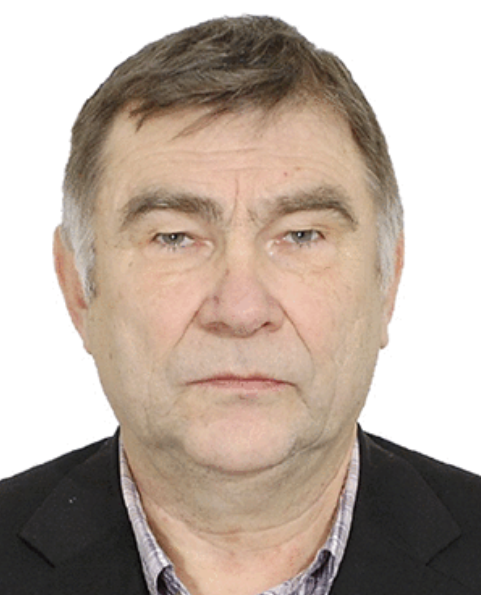
\includegraphics[width=1in,height=1.25in,clip,keepaspectratio]{images/bio/vd_pic.PNG}}]{VICTOR DUBININ} received the Diploma degree
in computer engineering, and the Ph.D. degree in
computer engineering and Dr.Sc. degree in computer science from the University of Penza, Penza,
Russia, in 1981, 1989, and 2014, respectively.
From 1981 to 1989, he was a Researcher, from
1989 to 1995, he was a Senior Lecturer, and from
1995 to 2015, he was an Associate Professor with
the University of Penza. Since 2015, he has been
a Professor with the Department of Computer Science, University of Penza. In 2011, he held a Visiting Researcher position with The University of Auckland, Auckland, New
Zealand, and from 2013 to 2019, he was with the Luleå University of Technology, Luleå, Sweden. His research interests include formal methods for
specification, verification, synthesis, and implementation of distributed and CPS. He was a recipient of DAAD-grants to work as a Guest Scientist with
Martin-Luther-University Halle-Wittenberg, Halle, Germany, in 2003, 2006,
and 2010, respectively.
\end{IEEEbiography}

\begin{IEEEbiography}[{
\includegraphics[width=1in,height=1.25in,clip,keepaspectratio]{images/bio/sandeep.jpeg}}]{SANDEEP PATIL} (S’11, M’19) received a Bachelor’s degree in computer science engineering from the CMR Institute of Technology, Bangalore, India, in 2005; a Master of computer science (software engineering) degree from the Illinois Institute of Technology, Chicago, IL, USA, in 2010; the Master of Engineering Studies (computer systems) degree from the University of Auckland, Auckland, New Zealand, in 2011; and a Ph.D. degree in formal verification of cyber-physical systems from the Lulea University of Technology, Lulea, Sweden. His research interests include software engineering principles and methodologies in distributed industrial automation, especially using the IEC 61499 paradigm. He also works with formal verification techniques in the same application field. He is an accomplished software engineering professional with over 16 years of research and development experience in systems and application software, including four years as a Senior Software Engineer at Motorola India Pvt. Ltd., India.
\end{IEEEbiography}


\begin{IEEEbiography}[{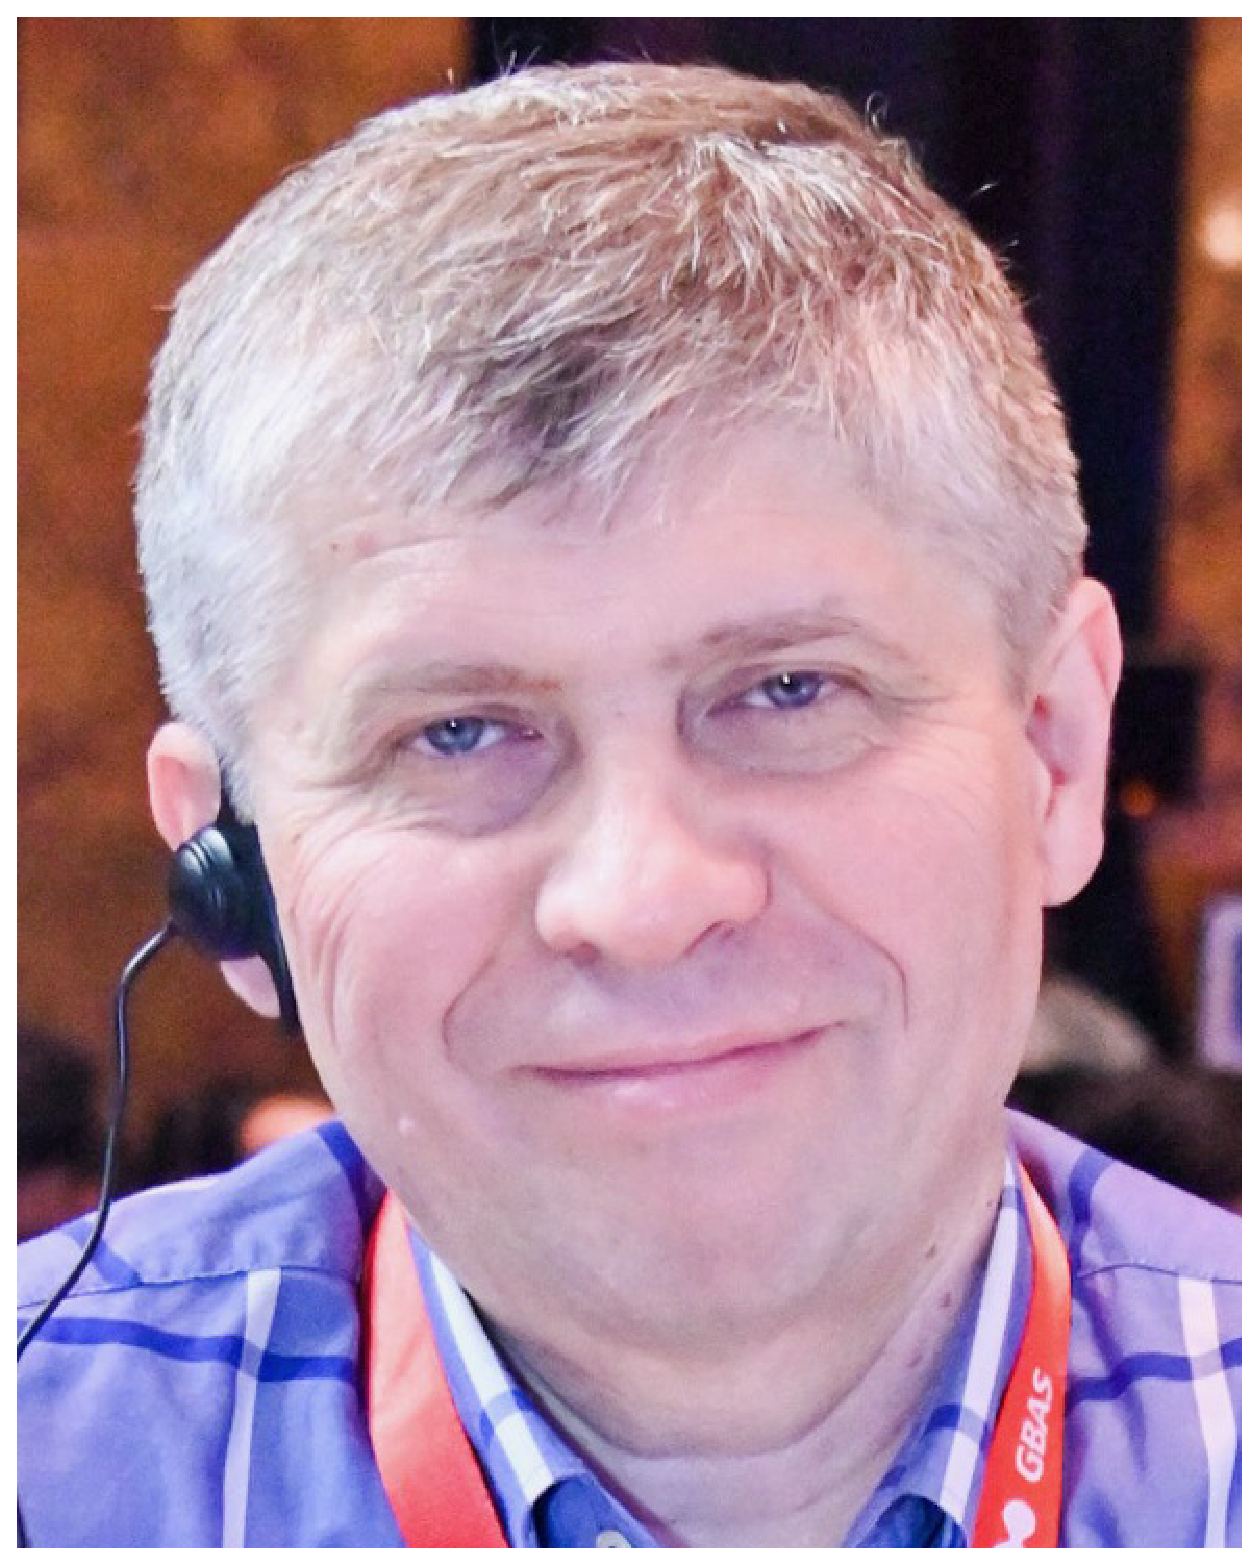
\includegraphics[width=1in,height=1.25in,clip,keepaspectratio]{images/bio/vyatk.eps}}]{Valeriy Vyatkin} (Fellow, IEEE) received Ph.D. degrees in Russia and Japan, in 1992 and 1999, respectively, and the Habilitation degree in Germany, in 2002., He is currently on Joint Appointment as the Chaired Professor with the Luleå University of Technology, Luleå, Sweden, and a Full Professor with Aalto University, Helsinki, Finland. Previously, he was a Visiting Scholar at Cambridge University, Cambridge, UK, and had permanent academic appointments with New Zealand, Germany, Japan, and Russia. His research interests include dependable distributed automation and industrial informatics, software engineering for industrial automation systems, artificial intelligence, distributed architectures, and multi-agent systems applied in various industry sectors, including smart grid, material handling, building management systems, data centres, and reconfigurable manufacturing. Dr. Vyatkin was a recipient of the Andrew P. Sage Award for the Best IEEE Transactions Paper in 2012. He has been Chair of the IEEE IES Technical Committee on Industrial Informatics since 2016 and Vice President of IES for Technical Activities for the term 2022–2025.
\end{IEEEbiography}

\EOD

\end{document}
